\documentclass[a4paper,11pt]{article}
\usepackage{newtxtext,newtxmath, amsmath, amsfonts, bm,mathtools}
\usepackage{paralist, url, natbib, parskip}
\usepackage{graphicx, subfig, adjustbox, todonotes}
\usepackage[section]{placeins}
\usepackage[linesnumbered,lined,boxed,commentsnumbered]{algorithm2e}
\usepackage[margin=1.5cm, bottom=2cm]{geometry}
\usepackage[margin=2cm]{caption}
\DeclareCaptionStyle{italic}[justification=centering]{labelfont={bf},textfont={it},labelsep=colon}
\captionsetup[figure]{style=italic,format=hang,singlelinecheck=true}

\SetKwInOut{Parameter}{parameter}
\setlength{\algomargin}{2em}
\renewcommand{\familydefault}{ptm}
\newcommand{\dist}{\text{dist}}
\newcommand{\diag}{\text{diag}}
\DeclareMathOperator{\sign}{sign}
\mathtoolsset{showonlyrefs}

\graphicspath{{./Graphics/}}

\allowdisplaybreaks

% =======================================================================
\begin{document}
% =======================================================================

\title{Dimension reduction for outlier detection using DOBIN}
\author{Sevvandi Kandanaarachchi, Rob J. Hyndman}
\maketitle

\begin{abstract}
	This paper introduces DOBIN, a new approach to select a set of basis vectors tailored for outlier detection. DOBIN has a solid mathematical foundation and can be used as a dimension reduction tool for outlier detection tasks. We demonstrate the effectiveness of DOBIN on an extensive data repository, by comparing the performance of outlier detection methods using DOBIN and other bases. We further illustrate the utility of DOBIN as an outlier visualization tool. The R package \textit{dobin} implements this basis construction.
\end{abstract}

% =======================================================================
\section{Introduction}
% =======================================================================

Outlier detection is used in diverse applications such as the identification of extreme weather events, stock market crashes and fraudulent transactions. A common challenge in many domains is that a data point may be an outlier in the original high dimensional space, but not an outlier in the low dimensional subspace created by a dimension reduction method.

We address this challenge by proposing a set of basis vectors tailored for unsupervised outlier detection which we call DOBIN: a Distance based Outlier BasIs using Neighbours. The acronym DOBIN is inspired from the informal verb `dob in', which the Collins English dictionary defines as `to inform against or report, specially to the police'. We emphasize that DOBIN is not an outlier detection method; rather it is a pre-processing step that can be used by any outlier detection method.

To the best of our knowledge no formal dimension reduction techniques exist for outlier detection. It is common to use Principal Component Analysis (PCA) where dimension reduction is used when detecting outliers \citep[e.g.,][]{talagala2019anomaly, hyndman2015large}. However, the goal of PCA is to find a set of basis vectors that explains the variance of the data, such that the highest variance is in the direction of the first vector, and so on. Therefore, the PC basis may not be suited for detecting outliers. By introducing DOBIN, we aim to bridge this gap in the literature.

We envisage two uses of DOBIN. First, as a basis more conducive to outlier detection, it brings outliers to the forefront using a smaller number of components. In this sense, it is somewhat similar to subspace outlier detection \citep[e.g.,][]{aggarwal2001outlier, keller2012hics}, although DOBIN does not detect outliers directly. If outliers arise in the full input space, DOBIN enables the outlier detection algorithm to detect outliers using fewer components. The second use of DOBIN is to assist with visualisation of outliers as we will see in Section~\ref{sec:ResWithVis}.

The literature on outlier detection has evolved in two fields, with contributions from statisticians and computer scientists. Although the methodologies used by the two groups are somewhat different, both groups have contributed to a rich and diverse literature, benefiting the broader community. Useful summaries of the computer science literature are provided by \citet{goldstein2016comparative} and \citet{zimek2012survey}; while similar surveys of the statistics outlier literature are given in \citet{rousseeuw2005} and \citet{unwin2019multivariate}. We have included methods from both disciplines in this paper.

Some methods treat outlier identification as a binary rule, with observations classified as outliers or otherwise \citep[e.g.,][]{billor2000bacon, wilkinson2017visualizing, rousseeuw2018detecting}, while other methods rank all observations in terms of ``outlyingness'' \citep[e.g.,][]{breunig2000lof, liu2008isolation}, or provide a probability of an observation being an outlier \citep[e.g.,][]{kriegel2009loop}. This difference impacts the performance evaluation metrics. Metrics such as false negatives and false positives or positive predictive value and negative predictive value are used to evaluate the binary results \citep{wilkinson2017visualizing}. By contrast, having a ranking of the observations leads to use tools such as area under the Receiver Operator Characteristic (ROC) curve, area under the Precision-Recall (PR) curve or precision at $n$ to evaluate performance \citep{campos2016evaluation}.

In Sections~\ref{sec:synthetic} and~\ref{sec:DatRepo} we investigate the effect of DOBIN on three outlier detection methods which first appeared in the computer science literature: LOF \citep{breunig2000lof}, KNN \citep{ramaswamy2000efficient} and iForest \citep{liu2008isolation}. To evaluate their performance, we use area under the ROC curve. We examine the effectiveness of DOBIN by comparing it against two other bases: PCA and the original basis. In Section~\ref{sec:synthetic} we use synthetic data to conduct experiments and in Section~\ref{sec:DatRepo} we use real data from our repository of more than $12,000$ datasets \citep{datasets}.

Section~\ref{sec:ResWithVis} examines outlier detection methods developed by the statistical community on some associated datasets. We use O3 plots by \cite{unwin2019multivariate}, which can be used to compare the results of six different outlier detection methods: \textit{HDoutliers} \citep{wilkinson2017visualizing}, \textit{mvBACON} \citep{billor2000bacon}, \textit{adjOutlyingness} \citep{brys2005robustification}, \textit{covMcd} \citep{rousseeuw1999fast} , \textit{FastPCs} \citep{vakili2014finding} and \textit{DetectDeviatingCells} \citep{rousseeuw2018detecting}. We use O3 plots in conjunction with the first two DOBIN components of each dataset and visually inspect if the outliers identified by the O3 plots are further away from the other points in the DOBIN space. This section highlights the usage of DOBIN as an outlier visualization tool.

We have produced an R package \textit{dobin} \citep{dobin}, which computes the DOBIN basis. In addition, all examples in this paper are available in the supplementary materials at \url{https://github.com/sevvandi/Outlier-Basis}. We start the next section with the mathematical framework of DOBIN. % in Section~\ref{sec:MathFrame}.

% =======================================================================
\section{Mathematical Framework}\label{sec:MathFrame}
% =======================================================================

Let $X_{N \times p}$ be a matrix denoting a dataset of $N$ observations and $p$ attributes. Let us denote the $i^{\text{th}}$ row of $X$ by $\bm{x}_i$. The distance between the observations $\bm{x}_i$ and $\bm{x}_j$ can be written as
\begin{equation}\label{eq:secMF1}
	\dist(\bm{x}_i, \bm{x}_j)^2 = ( \bm{x}_i - \bm{x}_j)^\top S ( \bm{x}_i - \bm{x}_j ) \, ,
\end{equation}
where $S$ is a symmetric positive definite matrix. In addition when $S$ is diagonal, i.e.\ $S = \diag(s_1, s_2, \dots, s_p)$, we obtain
\begin{equation}\label{eq:secMF2}
	\dist(\bm{x}_i, \bm{x}_j)^2 = \left\langle \eta\, , ( \bm{x}_i - \bm{x}_j )\circ ( \bm{x}_i - \bm{x}_j ) \right\rangle \,,
\end{equation}
where $\langle \cdot\, , \cdot \rangle$ denotes the standard inner product in $\mathbb{R}^p$, $\eta = (s_1, s_2, \dots, s_p)^\top$, and $\circ$ denotes the element-wise vector product. As $S$ is symmetric and positive definite it is diagonalizable, thus giving us motivation for considering a diagonal $S$.

\subsection{The $Y$ space}\label{sec:MathFrame1}

Next we establish the $Y$ space, which is instrumental in the construction of DOBIN\@. Let $\bm{y}_{ij} = ( \bm{x}_i - \bm{x}_j )\circ ( \bm{x}_i - \bm{x}_j ) = \left( ( x_{i1} - x_{j1} )^2, ( x_{i2} - x_{j2} )^2, \dots, \, ( x_{ip} - x_{jp} )^2 \right)$. Substituting in equation~\eqref{eq:secMF2} gives
\begin{equation}\label{eq:secMF3}
	\dist(\bm{x}_i, \bm{x}_j)^2 = \langle \eta\, , \bm{y}_{ij} \rangle\, .
\end{equation}
By finding the appropriate $\eta$ of unit length, we can maximize the distance between $\bm{x}_i$ and $\bm{x}_j$. This prompts the question as to which $\bm{x}_i$ and $\bm{x}_j$ need to be chosen to maximize the distance between them, if outlier detection is the goal. If we use knn distances as a guiding principle, we are interested in the $k$ nearest neighbours of a given point. Consequently, we can choose $\bm{x}_i$ and $\bm{x}_j$ that share a common neighbourhood.

If we were to calculate $\bm{y}_{ij}$ for all pairs, it would be computationally expensive as there are $N(N+1)/2$ pairs to consider. In addition, this would give us pairwise distances between points that we are not interested in, such as points on the boundary of the point cloud, that are opposite each other. Finding $\eta$ that maximizes the distances between such points is not beneficial for outlier detection, because a large distance between polar-opposite points does not mean that either of those points are outliers. Therefore we do not compute $\bm{y}_{ij}$ for all pairs of $\bm{x}_i$ and $\bm{x}_j$; rather we select the pairs that we want to include in our $Y$ space.

For each point $\bm{x}_i$ we compute $\bm{y}_{ij}$ arising from a set a nearest neighbours. From \cite{kandanaarachchi2018normalization} we know that nearest neighbours depend on the normalization technique. As a result, we choose two normalization techniques to pre-process the data; Min-Max and Median-IQR. Min-Max normalization scales each column to values between $0$ and $1$, with the minimum mapped to $0$ and the maximum mapped to $1$. Median-IQR scales each column to median $0$ and IQR $1$. Let $X_1$ denote the normalized data using Min-Max and $X_2$ using Median-IQR. For each normalization technique we choose a set of nearest neighbours from $k_1$ to $k_2$, that is for any point $\bm{x}_i$ we choose the $k_1^{\text{th}}$ nearest neighbour to the $k_2^{\text{th}}$ nearest neighbour. Here $k_1$ and $k_2$ are parameters and one can choose $k_1 =1$.

Next, for each point we find the union of nearest neighbours computed using the two normalization techniques. For example, for a given point $\bm{x}_i$, if the nearest neighbours according to Min-Max are $\{\bm{x}_2, \bm{x}_5, \bm{x}_9 \}$ and Median-IQR gives $\{\bm{x}_4, \bm{x}_5, \bm{x}_7 \}$, then we consider the union of these two sets as the set of nearest neighbours of $\bm{x}_i$. Using the nearest neighbours we construct a list of pairs denoted by $T$. Continuing the same example, the pairs $(\bm{x}_i, \bm{x}_2)$, $(\bm{x}_i, \bm{x}_4)$, $(\bm{x}_i, \bm{x}_5)$, $(\bm{x}_i, \bm{x}_7)$, $(\bm{x}_i, \bm{x}_9)$, and so on will be in $T$.

For each pair in $T$, we compute $\bm{y}_{ij}$ as in equation~\eqref{eq:secMF2} on the normalized space $X_1$ or $X_2$, depending on user preference. We now have the initial $Y$ space: a set of $\tilde{M}$ points in $\mathbb{R}^{p+}$. As the list of pairs that give rise to the initial $Y$ space are contained in $T$, we can denote $Y = \{ \bm{y}_\ell \}_{\ell=1}^{\tilde{M}}$, where each $\bm{y}_\ell = \bm{y}_{i_{(\ell)} j_{(\ell)} }$, i.e.\ $\ell$ is the row number in the matrix $Y$ and each $\bm{y}_\ell$ comes from the $\ell^{\text{th}}$ pair in $T$.

We are interested in neighbouring distances that are relatively large. The Euclidean distance squared between two points in the $X_1$ or $X_2$ space can be written as $\sum_{m=1}^p y_{\ell m}$ for the appropriate $\ell$. In order to consider only points with relatively large distances, we remove points that contribute to distances below a certain threshold determined by a percentile, i.e.\ we remove points such that $\sum_{m=1}^p y_{\ell m} < Q$ where $Q$ is the $q^{\text{th}}$ percentile of $ \left \{\sum_{m=1}^p y_{\ell m} \right \}_{\ell=1}^{\tilde{M}}$. We remove the associated pairs from $T$ as well. This constitutes the $Y$ space: $Y = \{\bm{y}_\ell \}_{\ell=1}^M$.

The main advantage of the $Y$ space is that it makes distance computation between two points in the $X$ space a linear function. This makes maximizing distances between points a much easier task.
Algorithm~\ref{algo:YSpace} summarizes the construction of the $Y$ space.

\DontPrintSemicolon
\begin{algorithm}\fontsize{9}{10}\selectfont
	\SetKwInOut{Input}{input~~~}
	\SetKwInOut{Output}{output}
	\Input{~$X$, $k_1, k_2 \in \mathbb{Z}^+$, $q \in (0, 1)$ and choice of normalization.}
	\Output{~The space $Y$ consisting of all $\{\bm{y}_\ell \}_{\ell=1}^M$ and the associated indices $i$ and $j$.}
	Normalize $X$ using Min-Max normalization. Let us call this space $X_1$. \\
	Find $k_1$ to $k_2$ nearest neighbours for each point in $X_1$. \\
	Next normalize $X$ using Median-IQR normalization. Let us call this space $X_2$. \\
	Find $k_1$ to $k_2$ nearest neighbours for each point in $X_2$. \\
	Then for each point collate all unique neighbours from both Min-Max and Median-IQR normalization methods. \\
	Let $T = $ the set of $i$ and $j$ indices, corresponding to the pairs of points in $X$. \\
	For all these pairs, compute $\bm{y}_{ij}$ as in equation~\eqref{eq:secMF3} using $X_1$ or $X_2$ space according to the choice of normalization. Let $Y =\big\{ \bm{y}_{1} =\bm{y}_{i_{(1)}j_{(1)}} , \bm{y}_{2} =\bm{y}_{i_{(2)}j_{(2)}}, \dots, \bm{y}_{\tilde{M}} =\bm{y}_{i_{(\tilde{M})}j_{(\tilde{M})}} \big\}$, where $\big( i_{(1)},j_{(1)} \big)$ is the first $(i, j)^{\text{th}}$ pair in $T$. Consequently $Y$ is an $\tilde{M}\times p$ matrix, with the $\ell^{\text{th}}$ row denoted by $\bm{y}_\ell$.\\
	Let $Q$ be the $q^{\text{th}}$ percentile of $ \left\{\sum_{m=1}^p {y}_{\ell m}\right\}$. The quantity $\sum_{m=1}^p {y}_{\ell m}$ is the distance between points $\bm{x}_{i_{(\ell)}}$ and $\bm{x}_{j_{(\ell)}}$ in $X_1$ or $X_2$ space. \\
	Remove points for which $ \sum_{m=1}^p {y}_{\ell m} < Q $. \\
	Remove the associated pairs of $(i, j)$ from $T$. \\
	The remaining points constitute the $Y$ space: $Y = \{\bm{y}_\ell \}_{\ell=1}^M$.
	\caption{\itshape Construction of the $Y$ space.}
	\label{algo:YSpace}
\end{algorithm}

\begin{figure}[!ht]
	\centering
	\subfloat[][]{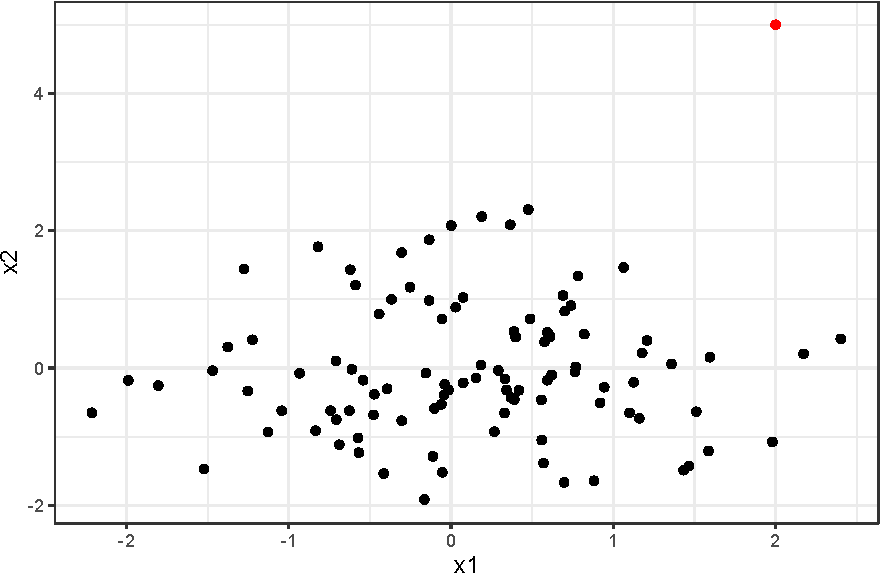
\includegraphics[width=0.48\textwidth]{X_space.pdf}\label{fig:XandY1}}\hfill
	\subfloat[][]{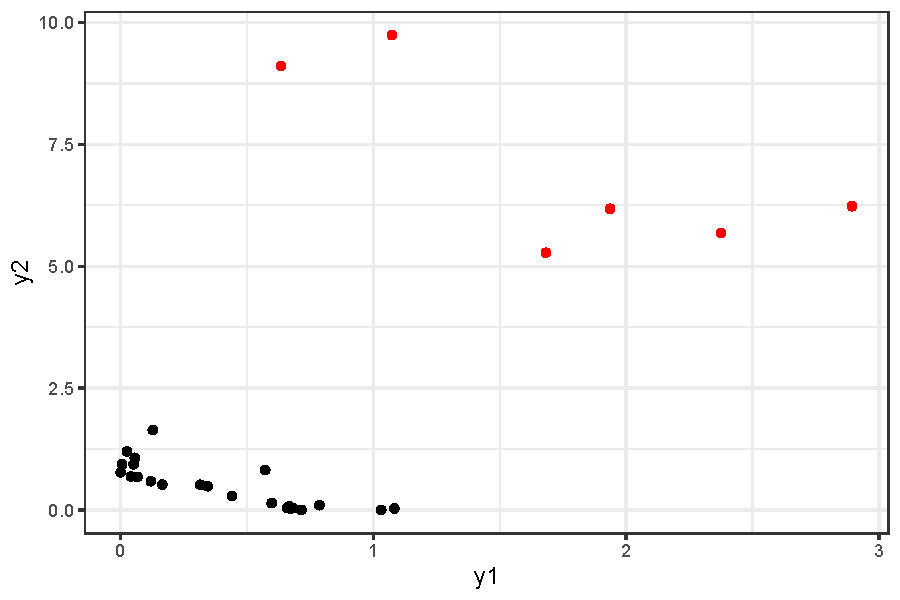
\includegraphics[width=0.48\textwidth]{Y_space.pdf}\label{fig:XandY2}}
	\caption{The $X$ and $Y$ spaces. The $X$ space in (a) and the associated $Y$ space in (b) with $q = 0.95$. The red coloured point in the $X$ space gives rise to 6 points, which are coloured in red in the $Y$ space.}
	\label{fig:XandY}
\end{figure}

%% Explanation of fig:XandY
Figure~\ref{fig:XandY} illustrates the $X$ and $Y$ spaces where $X$ is a 2 dimensional normal distribution of 100 points with a single outlier depicted in red. We see that the $Y$ space, computed with $k_1=1$ and $k_2=5$ consists of a lesser number of points compared to $X$, of which 6 points are contributed by the outlier. This is because $k_1$ to $k_2$ neighbours are considered in the construction of the $Y$ space and the points $\bm{y}_k$ with relatively small distances $\left(\sum_i y_{ki} \leq Q\right)$ are removed. Thus, the effect of outliers is magnified in the $Y$ space. %\todo{What is $k_1$ and $k_2$ in this example? - Done}

We summarise the salient features of the $Y$ space below:
\begin{compactenum}
	\item $Y = \{\bm{y}_\ell \}_{\ell=1}^M$, where $\bm{y}_\ell \in \mathbb{R}^{p+}$.
	\item Each $\bm{y}_\ell \in Y$ is constructed from two points $\bm{x}_i$ and $\bm{x}_j$ in $X$ with $T(\ell) = (i,j)$, where $T$ is a list consisting of the pairs in $X$ that are used to construct $Y$. In addition, $\bm{x}_i$ and $\bm{x}_j$ are $k$-nearest neighbours for some $k \in \{k_1, \dots, k_2\}$.
	\item For $i,j,\ell$ as above, $\bm{y}_\ell = (\bm{x}_i - \bm{x}_j) \circ (\bm{x}_i - \bm{x}_j) $, where $\circ$ denotes the element-wise vector product.
	\item The $Y$ space contains points $\bm{y}_\ell$ with relatively high $\sum_{m=1}^p y_{\ell m}$, i.e.\ it contains vectors that contribute to high knn distances in the $X$ space.
\end{compactenum}

\subsection{Maximising the distance between points}\label{sec:MathFrame2}

%The $Y$ space has points $\bm{y}_\ell$ that correspond to neighbouring points $\bm{x}_i$ and $\bm{x}_j$ in $X$, which have relatively high $k$ nearest neighbour distances.
Restating equation~\eqref{eq:secMF3} using $T(\ell) = (i,j)$ we obtain
\begin{equation} \label{eq:secMF4}
	\sum_{(i,j) \in T}\dist(\bm{x}_i, \bm{x}_j)^2 = \sum_{\ell}\langle \eta\, , \bm{y}_{\ell} \rangle\, .
\end{equation}
Thus the total distance squared for relatively high nearest neighbour distances $ \sum_{(i,j) \in T}\dist(\bm{x}_i, \bm{x}_j)^2$ can be maximised by finding the appropriate $\eta$ which maximises $\sum_{\ell}\langle \eta\, , \bm{y}_{\ell} \rangle$. However, \eqref{eq:secMF4} depends on the scale of $\eta$, so we normalize $\eta$ such that $ \lVert \eta \rVert = 1$. We now state our optimisation problem as
\begin{equation} \label{eq:secMF5}
	\max_\eta \sum_{\ell}\langle \eta\, , \bm{y}_{\ell} \rangle
  \qquad
	\text{subject to} \hspace{0.2cm} \lVert\eta\rVert^2 = 1 .
\end{equation}
Solving this using Lagrange Multipliers we obtain $\nabla f = \lambda \nabla g$, with
\begin{align}\label{eq:secMF6}
	f(\eta)  = \sum_{\ell}\langle \eta\, , \bm{y}_{\ell} \rangle \qquad \text{and} \qquad
	g(\eta) =  \lVert\eta\rVert^2 - 1 = 0 \, .
\end{align}
As $\nabla f = \left( \frac{\partial f}{\partial \eta_1}, \frac{\partial f}{\partial \eta_2}, \cdots, \frac{\partial f}{\partial \eta_p} \right)$ we compute
\begin{align}\label{eq:secMF7}
	\frac{\partial f}{\partial \eta_j}
     = \frac{\partial }{\partial \eta_j}\sum_{\ell}\langle \eta\, , \bm{y}_{\ell}\rangle
     = \frac{\partial }{\partial \eta_j} \sum_{\ell=1}^M \sum_{i=1}^p \eta_i y_{\ell i}
     = \sum_{\ell=1}^M \sum_{i=1}^p \delta_{ij} y_{\ell i}
     = \sum_{\ell=1}^M y_{\ell j} \, ,
\end{align}
where $\delta_{ij}$ is the Kronecker delta function which equals 1 when $i=j$ and zero otherwise. Hence
\begin{equation}\label{eq:secMF8}
	\nabla f = \left(\sum_{\ell=1}^M y_{\ell1}, \sum_{\ell=1}^M y_{\ell2}, \dots, \sum_{\ell=1}^M y_{\ell p} \right) = \sum_{\ell=1}^M \bm{y}_\ell \, .
\end{equation}
Similarly, as $g(\eta) = \left( \sum_{j=1}^p \eta_j^2\right) - 1$, we get $\nabla g = \eta$. By substituting $\nabla f = \lambda \nabla g$ and using $\lVert\eta\rVert = 1$, we obtain
\begin{equation}\label{eq:secMF9}
	\eta = \frac{\sum_{\ell=1}^M \bm{y}_\ell }{ \left\lVert\sum_{\ell=1}^M \bm{y}_\ell \right\rVert } \, .
\end{equation}

\subsection{Constructing a basis}\label{sec:MathFrame3}

We have computed the vector $\eta$ that maximises $\sum_{\ell}\langle \eta\, , \bm{y}_{\ell}\rangle$. To find a basis, we need to find the second, third and subsequent vectors which are orthogonal and in some way maximise the quantity $\sum_{\ell}\langle \eta\, , \bm{y}_{\ell}\rangle$. Let us first rename $\eta$ as $\eta_1$. Taking $\eta_1$ as the first basis vector, we take the projection of vector $\bm{y}_\ell$ on to $\eta_1$ and remove these components from $\bm{y}_\ell$:
\begin{equation}\label{eq:secMF10}
	\bm{y}_{\ell_1} = \bm{y}_\ell - \langle \eta_1 \, , \bm{y}_\ell \rangle \eta_1.
\end{equation}
Thus $\bm{y}_{\ell_1} \perp \eta_1$. Let $Y_1 = \{\bm{y}_{\ell_1} \}_{\ell=1}^M $ be the set of remaining components of $\{ \bm{y}_\ell \}_{\ell=1}^M$ after removing the projection on to $\eta_1$. Now we can compute $\eta_2$ which maximises $\sum_{\ell}\langle \eta\, , \bm{y}_{\ell_1}\rangle$ as
\begin{equation}\label{eq:secMF11}
	\eta_2 = \frac{\sum_{\ell=1}^M \bm{y}_{\ell_1} }{ \left\lVert\sum_{\ell=1}^M \bm{y}_{\ell_1} \right\rVert }\,.
\end{equation}
Proceeding in this way we obtain
\begin{align}
	\bm{y}_{\ell_{b}} & = \bm{y}_{\ell_{b-1}} - \langle \eta_b \, , \bm{y}_{\ell_{b-1}} \rangle \eta_b \, , \label{eq:secMF12} \\
	\text{and}\qquad \eta_{b+1}     & = \frac{\sum_{\ell=1}^M \bm{y}_{\ell_b} }{ \left\lVert\sum_{\ell=1}^M \bm{y}_{\ell_b} \right\rVert } \, , \label{eq:secMF13}
\end{align}
with $\bm{y}_{\ell_0} = \bm{y}_{\ell}$. The set $\Theta = \{ \eta_1, \eta_2, \dots , \eta_p \}$ gives a basis for $Y$ with each $\eta_{i+1}$ maximising $\sum_{\ell}\langle \eta\, , \bm{y}_{\ell_i} \rangle$. %which aims to maximise the quantity $\sum_{\ell}\left\langle \eta\, , \bm{y}_{\ell} \right\rangle$.
This process is somewhat similar to Gram Schmidt orthogonalisation.

Note that Equation~\eqref{eq:secMF4} is only true for $\bm{y}_\ell \in \mathbb{R}^{p+}$. The other $Y$ spaces $(Y_1, Y_2, \dots)$ are not subsets of $\mathbb{R}^{p+}$. To adjust for this, after computing $\bm{y}_{\ell_{b}}$ as in equation~\eqref{eq:secMF12}, we temporarily change the basis such that the points $\{\bm{y}_{\ell_{b}}\}_{\ell=1}^M$ are in a positive orthant. Then after computing $\eta_{b+1}$ as in equation~\eqref{eq:secMF13} using positive $\{\bm{y}_{\ell_{b}}\}_{\ell=1}^M$, we transform it back again to the original basis.

Once the basis $\Theta$ is computed, we change the basis of the original data as follows:
\begin{equation}\label{eq:secMF14}
	\tilde{X} = X_1 \Theta \, \hspace{0.5cm} \text{or} \hspace{0.5cm} \tilde{X} = X_2 \Theta
\end{equation}
where $X_1$ or $X_2$ is the normalized $X$ space according to the choice of normalization. We note that the basis $\Theta$ is not invariant to rotations; i.e.\ if one were to start with a different basis, the resulting $\Theta$ would be different. This is because when constructing the $Y$ space we compute element-wise squares of vector differences. While vector addition is basis invariant, squared element-wise components depend on the basis vectors. Notwithstanding this limitation, we achieve good results for experiments conducted on our extensive collection of more than $12,000$ real world datasets. For almost all of our experiments, we constructed DOBIN using the original basis as input. We only used a different basis if the number of variables were much higher than the number of observations. %DOBIN generally performs better with the original basis than with a transformed basis, and finds it is easier to compute the true direction of outliers when the axes are original variables, compared to when each axis is a linear combination of them.
Furthermore, as we will see in Section~\ref{sec:ResWithVis} it is easier to gain insights about the outlying directions when the axes are original variables.

We conclude this mathematical discussion by summarizing the key steps of DOBIN:
\begin{compactenum}
	\item Find the $Y$ space for a given dataset $X$ as detailed in Algorithm~\ref{algo:YSpace}.
	\item Construct the basis $\Theta$ as outlined in Section~\ref{sec:MathFrame3}.
	\item Transform the original space $X$ using equation~\eqref{eq:secMF14}.
\end{compactenum}

\subsection{Parameters of DOBIN}\label{sec:MathFrame4}

We have three numerical parameters $k_1$, $k_2$ and $q$ for constructing the $Y$ space with the following default values:
\begin{align} \label{eq:secMF15}
	k_2 & = \min\left(20, \max (\lfloor N/20 \rfloor ,2) \right) \notag \, , \\
	k_1 & = \max (k_2-10, 1) \, ,                                             \\
	q   & = 0.95 \notag \, ,
\end{align}
where $N$ is the number of observations in the dataset. The parameters $k_1$ and $k_2$ affect the run time of the algorithm, so we set a maximum value of $20$ for $k_2$. As $k_1 < k_2$, we consider a maximum of $10$ neighbours for each point. The parameter $q$ determines the cut-off quantile needed to obtain a subset of $\bm{y}$ with large distances. Therefore $q$ needs to be a relatively high value in the interval $(0,1)$. From equation~\eqref{eq:secMF5} we maximise the projection of $\bm{y}$ on to $\eta$. If $q$ is too low, many $\bm{y}$ with smaller projections may contribute heavily to the sum, making DOBIN vectors less effective.

The other parameter for constructing the $Y$ space is the choice of normalization. While Min-Max normalization is commonly used by the computer science community \citep{campos2016evaluation}, other normalization techniques such as distance from univariate medians and Mahalanobis distance are commonly used by the statistical community \citep{billor2000bacon}. We give two options for normalization: Min-Max and Median-IQR.

The purpose of the final parameter is to aid visualisation in two dimensions. As points $\{\bm{y}_{\ell}\}_{i=1}^M$ lie in the positive orthant, the first vector $\eta_1$ which maximizes $\sum_\ell \langle \eta\, \bm{y}_\ell\rangle$ also lies in the positive orthant. However, this may not render the best possible 2D-visualization of the outliers in $X$ space, because points can have positive and negative coordinates in $X$ space. Hence we compute the signed $\bm{y}_{\ell}$, denoted by $\bm{\tilde{y}}_\ell$, by keeping track of the signs of the point differences $(\bm{x}_i - \bm{x}_j)$. Let $T(\ell) = (i, j)$, then
\begin{equation}\label{eq:secMF16}
	\bm{\tilde{y}}_\ell = \sign(\bm{x}_i - \bm{x}_j) \circ \bm{y}_{\ell} \, ,
\end{equation}
where $\circ$ denotes element-wise multiplication. Then
\begin{align}\label{eq:secMF17}
	\sign(\eta_1) & = \sign \left( \sum_{i=1}^M \bm{\tilde{y}}_\ell \right) \, , \notag \\
	\text{and}\qquad
  \tilde\eta_1  & = \sign (\eta_1) \circ \eta_1,
\end{align}
where $\eta_1 $ is computed using equation~\eqref{eq:secMF9}. However, this adds to the computation and is only recommended if 2D-visualization is an aim of the exercise.

% =======================================================================
\section{Experiments with synthetic data}\label{sec:synthetic}
% =======================================================================

In this section we do three experiments with synthetic data. For each experiment we compare results for three outlier detection methods, namely LOF \citep{breunig2000lof}, KNN \citep{ramaswamy2000efficient} and isolation forest \citep{liu2008isolation}. We choose these methods as they are well recognised and fundamentally different: LOF uses a local density based approach; KNN uses a global distance based approach; and iForest uses a randomised tree based approach. For each outlier detection method we consider the following three coordinate systems:
\begin{enumerate}
	\item All variables in the dataset;
	\item Perform Principal Component Analysis (PCA) on the dataset, and use the first half of the principal components (PCs).
	\item Perform DOBIN on the dataset, and use the first half of the DOBIN components.
\end{enumerate}
For each outlier detection method, we compare the results using these three sets of coordinates. We use area under the Receiver Operator Characteristic curve (AUC) as our performance measure.

\subsection{Experiment 1}

The first experiment considers two normal distributions: an inlier normal distribution and an outlier normal distribution, which moves out from the inlier distribution as its mean increases. We consider a dataset of $405$ observations in $\mathbb{R}^6$, of which $400$ observations in each dimension are normally distributed with mean $0$ and standard deviation $1$. The remaining $5$ observations signify outliers and are normally distributed with mean $\mu$ and standard deviation $0.2$ in one dimension, and mean $0$ and standard deviation $1$ in other dimensions. The value of $\mu$ is changed from $0$ to $4.5$ by increments of $0.5$. The reason for a smaller standard deviation in the first dimension is to ensure that the outliers stay close to the mean $\mu$ and move out of the inlier distribution as $\mu$ increases. For each value of $\mu$ we consider the three sets of coordinates described above and their performance using the outlier methods LOF, KNN and iForest. We perform $10$ iterations of this experiment. Figure~\ref{fig:Exp1} shows the results for all three outlier methods using the average performance values of $10$ iterations.

Using $3$ DOBIN components gives the highest performance for all $3$ outlier detection methods for $\mu > 1$. Indeed, we are interested in a set of coordinates that can accentuate the outliers as they move out from the inlier distribution. For values of $\mu \in \{0, 0.5, 1\}$, the outlier distribution lies in the interior of the inlier distribution, making a performance comparison between the coordinates not meaningful.

\subsection{Experiment 2}

\begin{figure}[!p]
  \centering
  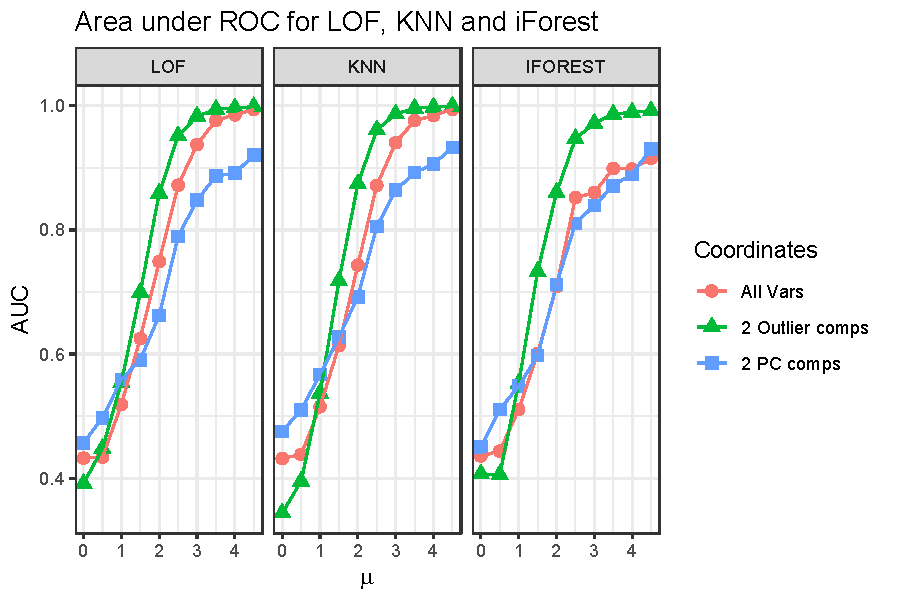
\includegraphics[width=0.6\textwidth]{Exp1.pdf}
  \caption{Results of Experiment 1, in $\mathbb{R}^6$.}
  \label{fig:Exp1}\vspace*{0.3cm}

  \centering
  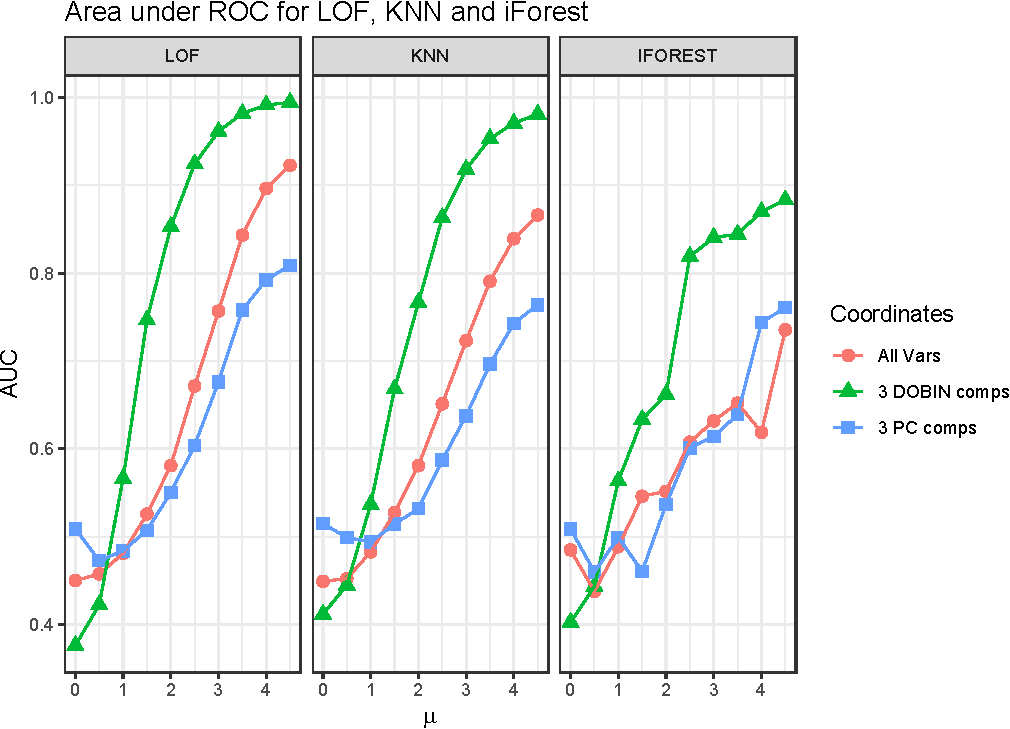
\includegraphics[width=0.6\textwidth]{Exp2.pdf}
  \caption{Results of Experiment 2, in $\mathbb{R}^6$.}
  \label{fig:Exp2}\vspace*{0.3cm}

  \centering
  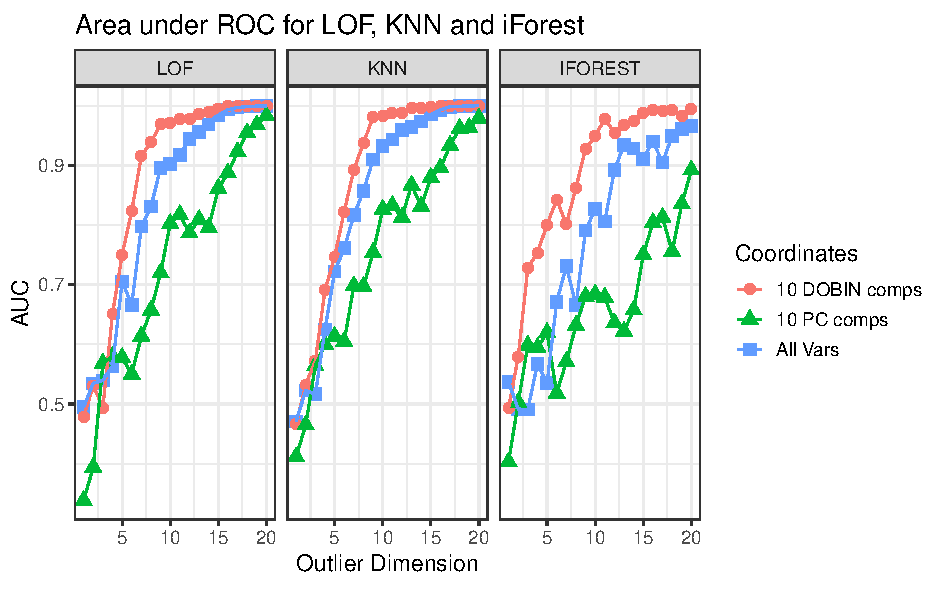
\includegraphics[width=0.6\textwidth]{Exp3.pdf}
  \caption{Results of Experiment 3, in $\mathbb{R}^{20}$.}
  \label{fig:Exp3}
\end{figure}

The second experiment considers a bi-modal setting with two inlier normal distributions and one outlier normal distribution which moves into the valley as its mean changes. Somewhat similar to the previous example we consider $805$ observations in $\mathbb{R}^6$; $800$ inlier observations of which $400$ centred at $(5,0,0,0,0,0)$ and the other $400$ centred at $(-5,0,0,0,0,0)$. All inlier observations come from normal distributions with standard deviation $1$ in each dimension. The outlier distribution consists of $5$ points with mean $(5-\mu,0,0,0,0,0)$ and standard deviations $0.2$ in the first dimension and $1$ in other dimensions. The value of $\mu$ is increased from $0$ to $4.5$ in increments of $0.5$. Again, a smaller standard deviation is to ensure that the outliers move into the valley. Figure~\ref{fig:Exp2} shows the results for all three outlier methods on all three coordinate systems using the average values of 10 iterations.

Again we see that using 3 DOBIN components gives the highest performance for all three outlier methods. %In particular,

\subsection{Experiment 3}

The third experiment is motivated from \cite{zimek2012survey}. We consider a uniform distribution in $\mathbb{R}^{20}$ and place a manual outlier at $0.9$ in $i$ dimensions where $i$ is changed from $1$ to $20$. While this is not an outlier in any single dimension, as $i$ increases this point stands out from the rest of the distribution. Indeed, for large $i$ this point lies furthest from the rest. An equivalent outlier is $0.1$ in $i$ dimensions. The reason that these points are outliers is because they are at the corners of the hyper-cube and so are far away from other points. On the contrary, $0.5$ in $i$ dimensions would be closest to other points. This is because $(0.5, 0.5, \dots)$ has neighbours from all sides and has on average $2^{20}$ more neighbours compared to $(1, 1, \dots)$ which is a corner on the unit hyper-cube. For practical purposes the point $(0.9, 0.9, \dots)$ is similar to $(1, 1, \dots)$ and has significantly less neighbours compared to $(0.5, 0.5, \dots)$. Figure~\ref{fig:Exp3} shows the results of all three outlier methods on all three coordinate systems. Again we see that using half of the DOBIN components gives the best performance for all three outlier methods.

In all three experiments we see that DOBIN coordinates give the best performance followed by the full set of coordinates. Principal Components are generally less effective than the full set of coordinates for these three experiments and outlier methods. We note that this is not a failure of PCA, as outlier detection is not its intended goal. Rather, PCA maximizes the variance in each component such that a low dimensional representation of the dataset is a good approximation to the original. These results suggest that DOBIN is preferred over PCA as a dimension reduction technique for outlier detection. % \citep{talagala2019anomaly, hyndman2015large}

% REDO EXPERIMENT 1 AND 2 WITH REFLE = FALSE
% =======================================================================
\section{Results with visualization}\label{sec:ResWithVis}
% =======================================================================

In this section we investigate specific examples motivated from \cite{unwin2019multivariate} and \cite{wilkinson2017visualizing} using O3 plots and the DC1-DC2 space, which is the space spanned by the first two DOBIN vectors. O3 plots \citep{unwin2019multivariate} can be used to compare the results of $6$ different outlier detection methods: \textit{HDoutliers}, \textit{mvBACON}, \textit{adjOutlyingness}, \textit{covMcd}, \textit{FastPCs}, and \textit{DetectDeviatingCells}. Besides facilitating an ensemble of outlier methods, O3 plots also highlight outliers in axis parallel subspaces. We use O3 plots as a means of validating the DC1-DC2 space.

\subsection{\textit{Election2005} dataset}\label{sec:ResWithVis1}

We start with the \textit{Election2005} dataset \citep{mbgraphic}, which is used by \cite{unwin2019multivariate} to illustrate the O3 plot. This dataset includes election results of two German elections and certain attributes of the electorates. We examine the O3 plot and the DC1-DC2 space of this dataset.

\begin{figure*}[!ht]
	\centering
	\subfloat[][]{
		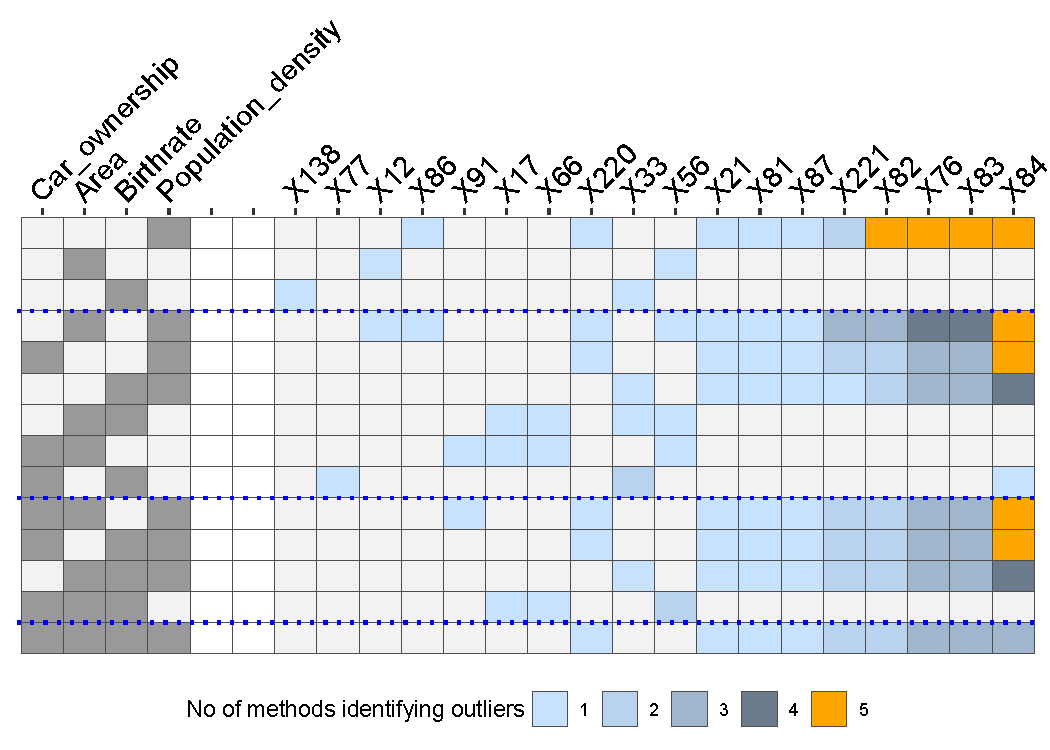
\includegraphics[width=0.54\textwidth]{Ex1_1.pdf}
		\label{fig:Election20051}
	}\hfill
	\subfloat[][]{
		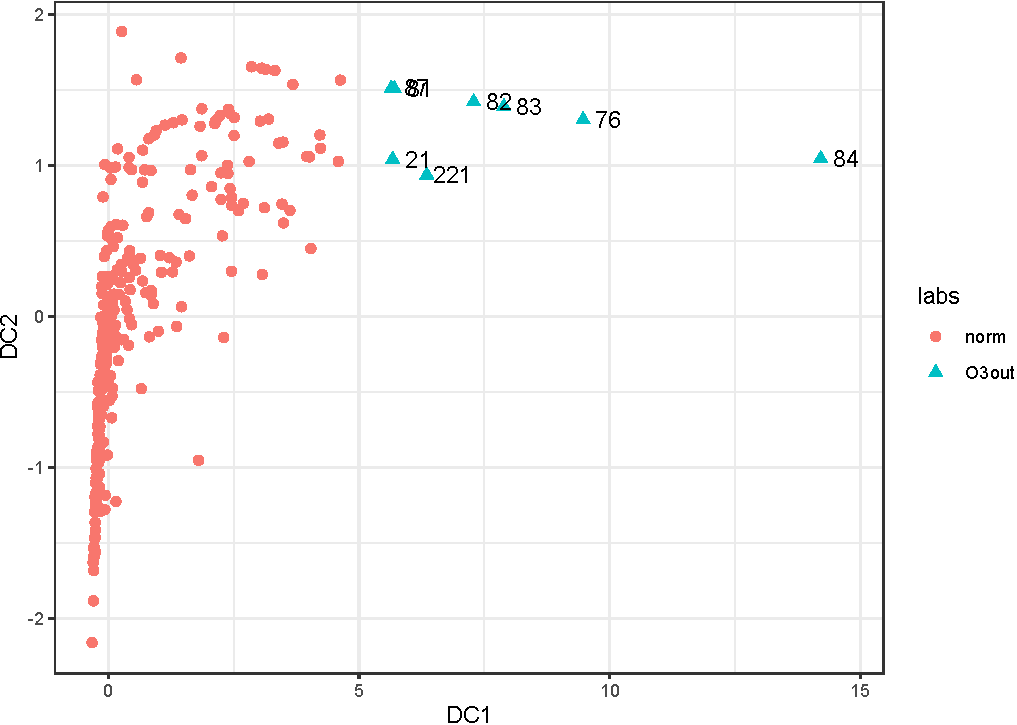
\includegraphics[width=0.43\textwidth]{Ex1_2.pdf}
		\label{fig:Election20052}
	}%
	\caption{O3plot of the \textit{Election2005} dataset in Figure~\ref{fig:Election20051} and the first 2 DOBIN components in Figure~\ref{fig:Election20052} }
	\label{fig:Election2005}
\end{figure*}

Figure~\ref{fig:Election20051} shows the O3 plot of this dataset using all six outlier methods. The columns on the left indicate the variables, the columns on the right indicate the observations, the rows specify the axis parallel subspaces and the colours depict the number of methods that identify each observation in each subspace as an outlier. From this plot we see that observation $X84$ is identified as an outlier by $5$ methods in $5$ subspaces, $4$ methods in $2$ subspaces, $3$ methods in $1$ subspace and by $1$ method in $1$ subspace. $X84$ is arguably the most outlying observation in this dataset. The observations $X83$, $X76$, $X82$ are also identified as outliers by $5$ methods in the dimension of population density. They are also identified as outliers by multiple methods in different subspaces. The layout of the O3 plot is such that the outlyingness of the observations increase to the right.

Figure~\ref{fig:Election20052} shows the first $2$ DOBIN components of the \textit{Election2005} dataset. This is a projection of the dataset onto a two dimensional subspace spanned by the first $2$ DOBIN vectors. Here we see the observation $X84$ (denoted by $84$ on the plot) far away from the rest of the data with $X76$, $X83$ and $X82$ somewhat detached from the rest. The observations $X87$ an $X81$ are almost at the same position in this $2$-dimensional space. The observations $X221$ and $X21$ also appear a bit outside the boundary of other points. A simple KNN algorithm in the DC1-DC2 space gives the top $8$ candidates as $X84$, $X76$, $X83$, $X82$, $X221$, $X81$, $X87$, and $X21$. Thus, the DC1-DC2 space accentuates the eight most outlying observations according to the O3 plot, while showing clearly that $X84$ is the most outlying observation.

The first DOBIN vector is of interest to us as the outliers deviate most in this direction. Equation~\eqref{eq:ResWithVis1} gives the first DOBIN vector, DC1, as a linear combination of the input variables.
\begin{equation}\label{eq:ResWithVis1}
	\text{DC1} = \begin{bmatrix}
		0.008 & 0.998 & 0.040 & -0.050
	\end{bmatrix}
	\begin{bmatrix}
		\text{Area}               \\
		\text{Population Density} \\
		\text{Birthrate}          \\
		\text{Car Ownership}
	\end{bmatrix}
\end{equation}
From equation~\eqref{eq:ResWithVis1} we see that \textit{Population Density} is the main variable contributing to outliers in the DC1-DC2 space. The O3 plot supports this observation. If we look carefully at the O3 plot we see that $X21$ to $X84$ gets identified as outliers in all subspaces that contain \textit{Population Density}. This insight gives us a better understanding of the dataset.

\subsection{\textit{Diamonds} dataset}\label{sec:ResWithVis2}

The next example is taken from the \textit{O3Outliers} R package \citep{O3Rpack} and uses the \textit{Diamonds} dataset \citep{ggplot2}. This dataset contains attributes of diamonds.

\begin{figure*}[!ht]
	\centering
	\subfloat[][]{
		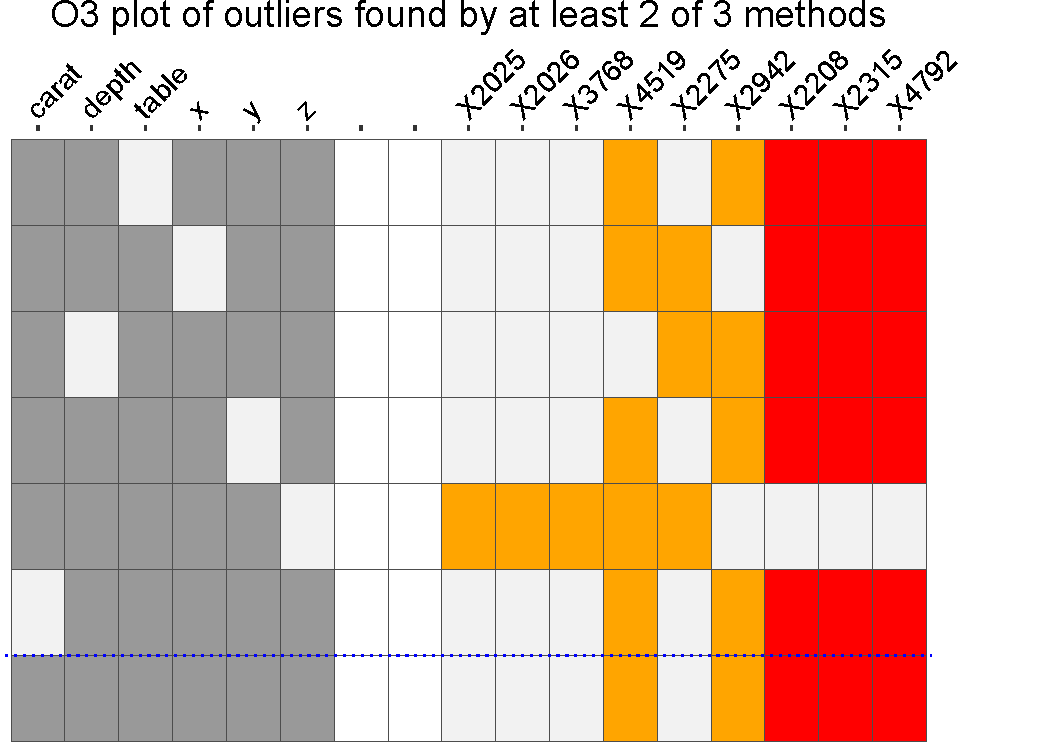
\includegraphics[width=0.45\textwidth]{Ex2_1.pdf}
		\label{fig:Diamonds1}
	}\hfill
	\subfloat[][]{
		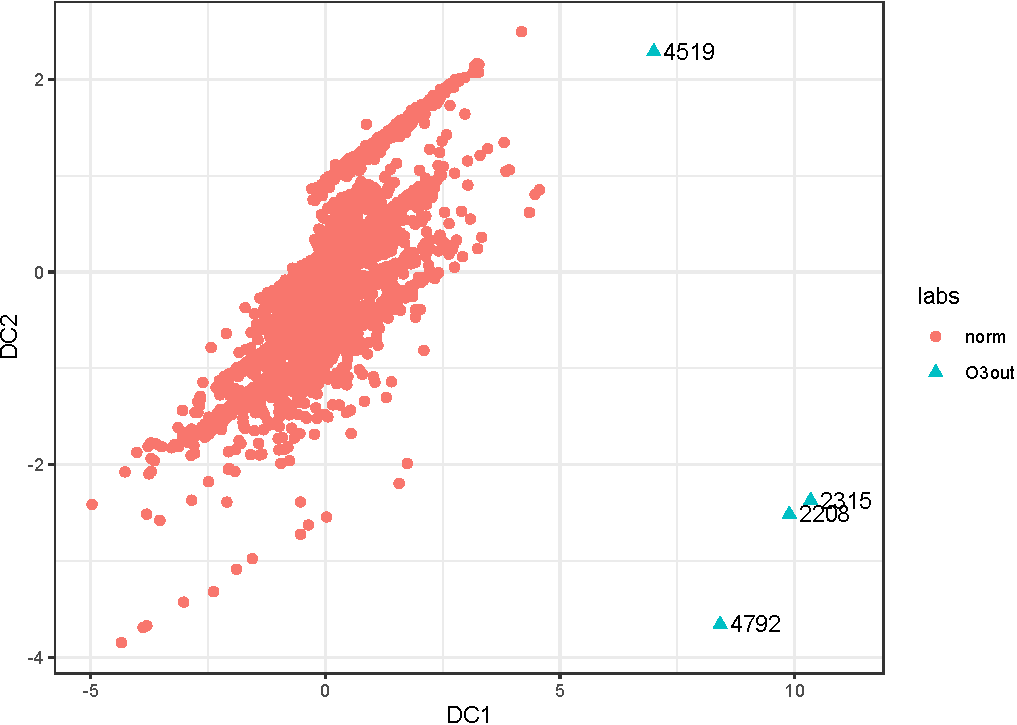
\includegraphics[width=0.43\textwidth]{Ex2_2.pdf}
		\label{fig:Diamonds2}
	}%
	\caption{O3plot of the \textit{Diamonds} dataset in Figure~\ref{fig:Election20051} and the first 2 DOBIN components in Figure~\ref{fig:Election20052}.}
	\label{fig:Diamonds}
\end{figure*}

Figure~\ref{fig:Diamonds1} shows the O3 plot of this dataset using the three outlier methods \textit{HDoutliers}, \textit{FastPCs} and \textit{adjOutlyingness}. We could not use all six methods on this dataset as the other three methods included in the \textit{OutliersO3} R package gave computational errors. Of the three methods used, all methods identified $X4792$, $X2315$ and $X2208$ as outliers in 6 subspaces including the full space. These $3$ points appear in the DC1-DC2 space in the bottom right corner. In addition, the point $X4519$ (denoted by $4519$ in the plot) appears in the top right corner in the DC1-DC2 space, away from other points. Comparing with the O3 plot, we see that $X4519$ is identified as an outlier by $2$ methods in $6$ subspaces. In keeping with the guidelines of the previous section, we use half of the DC components to evaluate a KNN algorithm. The top $4$ candidates in this $3$-dimensional DC space are $X4792$, $X2315$, $X2208$ and $X4519$ in that order.

To understand the first DOBIN vector, we look at its coefficients:
\begin{equation}\label{eq:ResWithVis2}
	\text{DC1} = \begin{bmatrix}
		0.098 & -0.659 & 0.185 & 0.097 & 0.126 & -0.704
	\end{bmatrix}
	\begin{bmatrix}
		\text{Carat} \\
		\text{Depth} \\
		\text{Table} \\
		\text{x}     \\
		\text{y}     \\
		\text{z}
	\end{bmatrix}
\end{equation}
We see that the variables \textit{z} and \textit{Depth} contribute more to outliers in the DC1-DC2 space as well as in the O3 plot.
%Thus the DOBIN basis can be used to project data for easy visualization of outliers.

\subsection{\textit{USArrests} dataset}\label{sec:ResWithVis3}

The popular \textit{USArrests} dataset is studied by \cite{bailey1995interactive, sarkar2008labels, yaminiviolent} and many others. This dataset contains violent crime rates for the 50 US states in 1973. The O3 plot using all six outlier detection methods and the DC1-DC2 space of this dataset are illustrated in Figure~\ref{fig:USArrests}.

\begin{figure*}[!ht]
	\centering
	\subfloat[][]{
		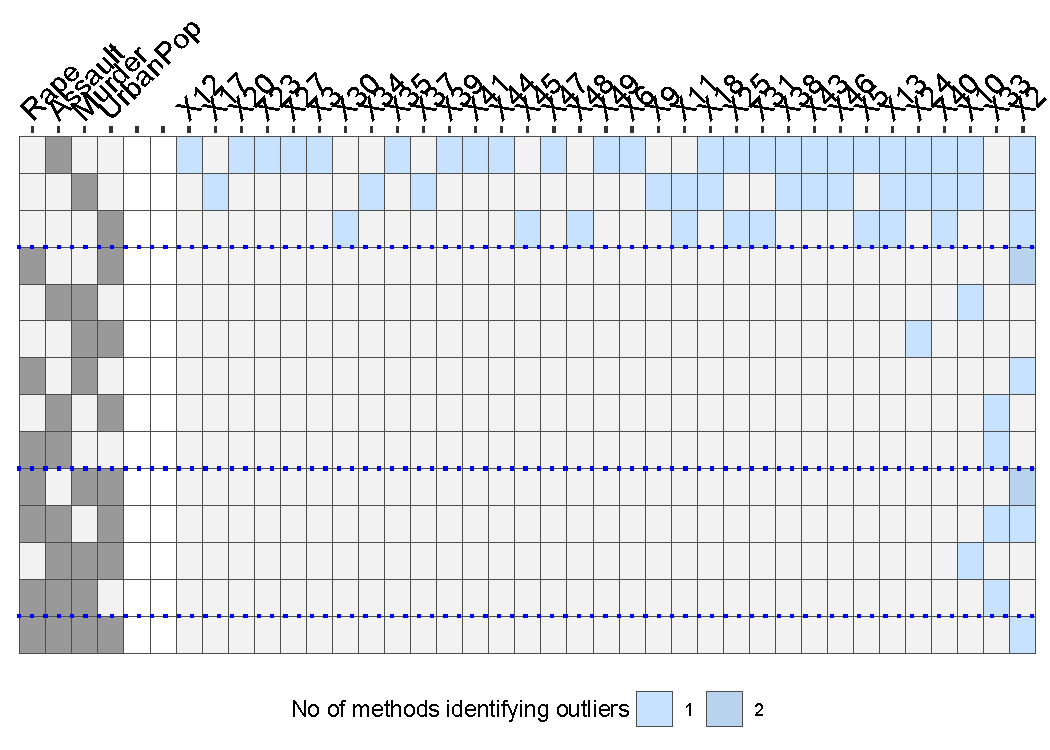
\includegraphics[width=0.52\textwidth]{Ex3_1.pdf}
		\label{fig:USArrests1}
	}\hfill
	\subfloat[][]{
		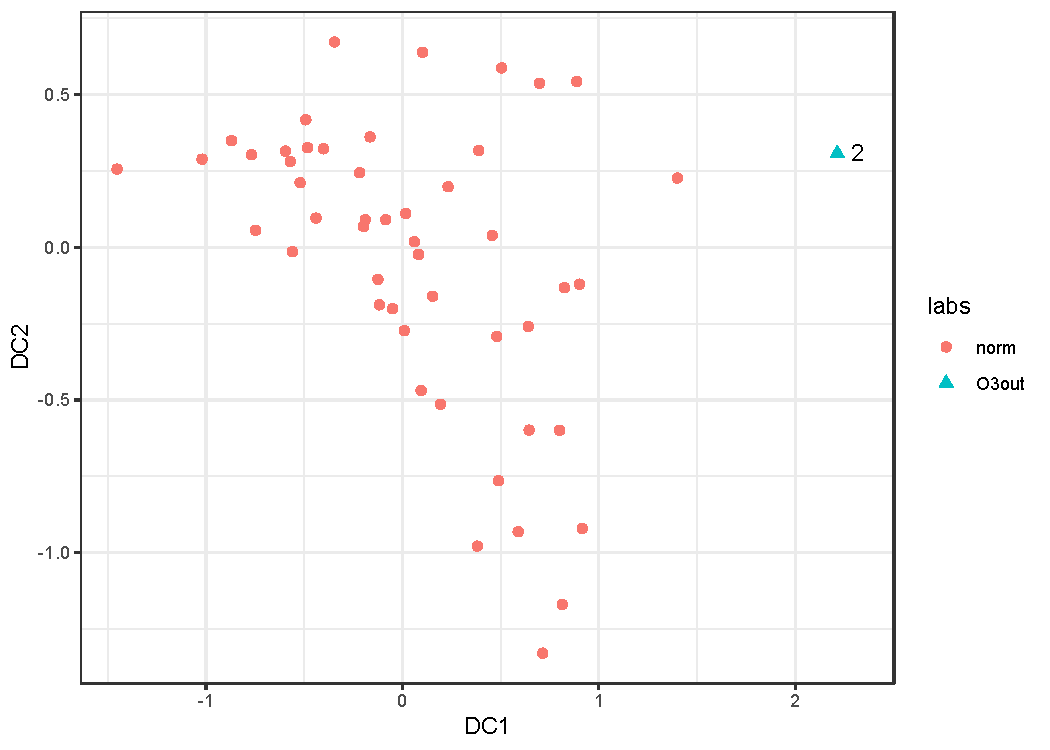
\includegraphics[width=0.43\textwidth]{Ex3_2.pdf}
		\label{fig:USArrests2}
	}%
	\caption{O3plot of the \textit{USArrests} dataset in Figure~\ref{fig:USArrests1} and the first 2 DOBIN components in Figure~\ref{fig:USArrests2}.}
	\label{fig:USArrests}
\end{figure*}

From Figure\ref{fig:USArrests1} we see that $X2$ (corresponding to Alaska) is flagged as an outlier in $8$ subspaces including the full space, by one or two outlier detection methods. The adjoining outlier $X33$ (North Carolina) is only flagged in $4$ subspaces and the others in even smaller subspaces. Of the six outlier methods, only two identify Alaska as an outlier in certain subspaces. This also suggests that even though there is consensus between two methods, as only one third of the methods agree on this outlier, it may not be quite so outlying as the outliers in the previous examples. Indeed, this notion is validated by the DC1-DC2 plot. We see the observation $X2$ (denoted by $2$ in the plot) standing out from the rest, but not by a large margin. A KNN algorithm identifies this observation as having the highest KNN distance in DC1-DC2 space.

We look at the coefficients of the first DOBIN vector as $X2$ deviates in DC1:
\begin{equation}\label{eq:ResWithVis3}
	\text{DC1} = \begin{bmatrix}
		0.173 & 0.077 & -0.675 & 0.713
	\end{bmatrix}
	\begin{bmatrix}
		\text{Murder}   \\
		\text{Assault}  \\
		\text{UrbanPop} \\
		\text{Rape}
	\end{bmatrix} \,
\end{equation}
We see that the variables \textit{UrbanPop} and \textit{Rape} contribute more to the first DOBIN vector than the other variables. From equation~\eqref{eq:ResWithVis3}, high values of DC1 indicate low percentages of urban population and high rape arrests per $100,000$ residents. Therefore, we might expect Alaska to have higher rape arrests per urban capita. Indeed from Figure~\ref{fig:USArrests3} we see that Alaska has the highest ratio of \textit{Rape/UrbanPop} of all $50$ states confirming the insight gleaned from the first DOBIN vector.

\begin{figure*}[!ht]
	\centering
	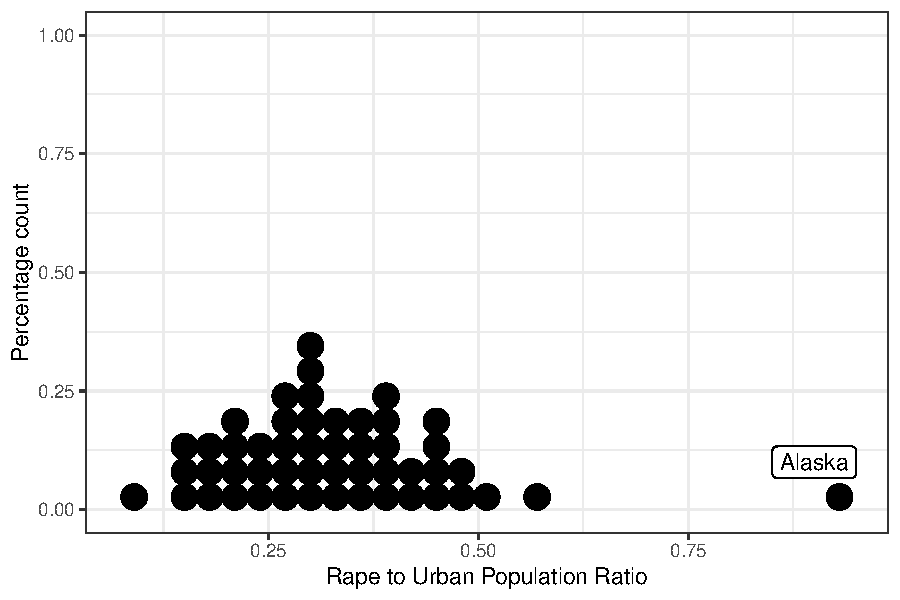
\includegraphics[width=0.6\textwidth]{Ex3_3.pdf}
	\caption{USArrests dataset -- Rape to Urban population ratio values.}
	\label{fig:USArrests3}
\end{figure*}

\subsection{\textit{Airquality} dataset}\label{sec:ResWithVis4}

The \textit{Airquality} dataset discussed in \cite{john1983graphical} has measurements on air quality in New York city from May to September 1973. The O3 plot using all $6$ outlier methods and the DC1-DC2 space of this dataset are shown in Figure~\ref{fig:Airquality}.

\begin{figure*}[!ht]
	\centering
	\subfloat[][]{
		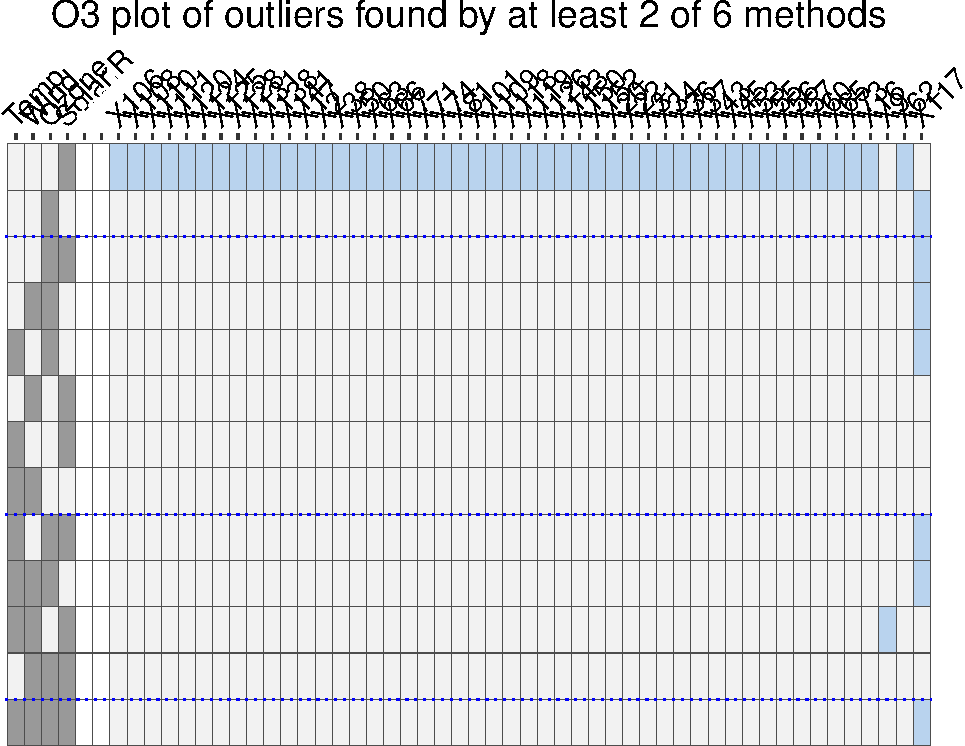
\includegraphics[width=0.54\textwidth]{Ex4_1.pdf}
		\label{fig:Airquality1}
	}\hfill
	\subfloat[][]{
		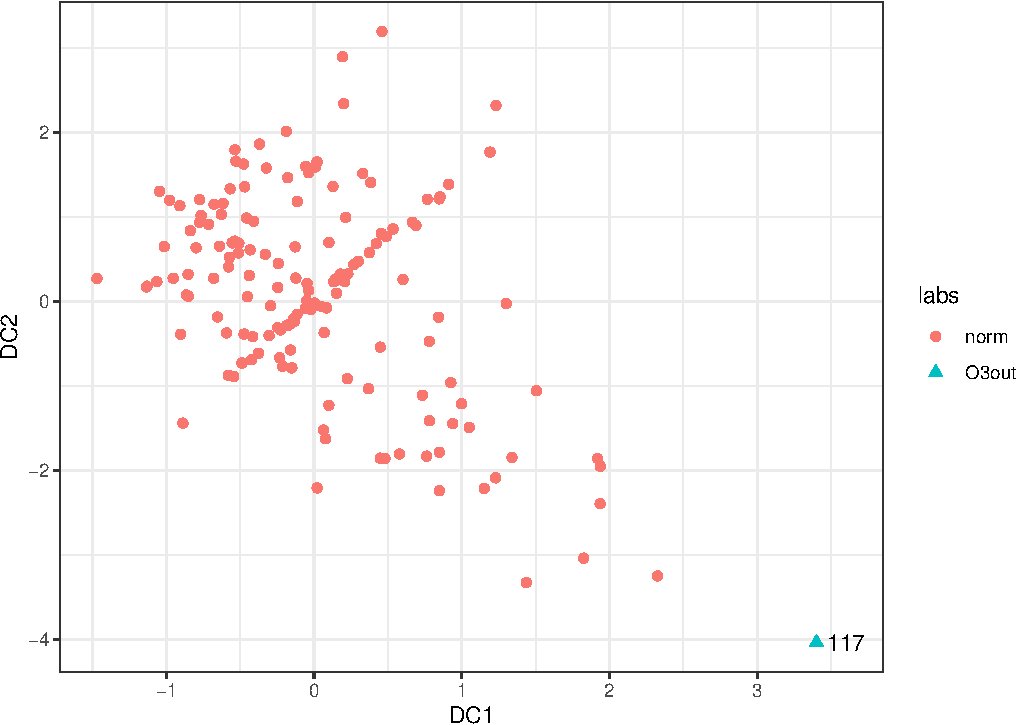
\includegraphics[width=0.43\textwidth]{Ex4_2.pdf}
		\label{fig:Airquality2}
	}%
	\caption{O3plot of the \textit{Airquality} dataset in Figure~\ref{fig:Airquality1} and the first 2 DOBIN components in Figure~\ref{fig:Airquality2}.}
	\label{fig:Airquality}
\end{figure*}
The O3 plot in Figure~\ref{fig:Airquality1} shows $X117$ as the only outlier identified in $6$ subspaces by $2$ methods. The associated DC1-DC2 space shows the observation $X117$ (denoted by $117$ in the plot) away from the rest at the bottom right. Again, we see agreement between the O3 plot and DC1-DC2 space. The observation $X117$ was identified as an outlier only by a third of the outlier methods. This is corroborated in the DC1-DC2 plot by comparatively less outlyingness of observation $X117$ compared to outliers in the \textit{Diamonds} dataset. Performing a KNN algorithm revealed the observation with the highest KNN distance as $X117$ in the DC1-DC2 space.

The first DOBIN vector has the following coefficients:
\begin{equation}\label{eq:ResWithVis4}
	\text{DC1} = \begin{bmatrix}
		0.842 & -0.078 & 0.512 & -0.151
	\end{bmatrix}
	\begin{bmatrix}
		\text{Ozone}   \\
		\text{Solar.R} \\
		\text{Wind}    \\
		\text{Temp}
	\end{bmatrix} \,
\end{equation}
From equation~\eqref{eq:ResWithVis4} we see that the observation $X117$ is an outlier due to high values of \textit{Ozone} and \textit{Wind}.

\subsection{\textit{lesmis} dataset}\label{sec:ResWithVis5}

The \textit{lesmis} dataset \citep{sombrero} contains the character coappearance network of characters in the novel \textit{Les Mis\'erables} by Victor Hugo. This dataset is stored as a graph, with vertices corresponding to characters and is shown in Figure~\ref{fig:lesmisgraph}. The character network in \textit{Les Mis\'erables} is also studied in \cite{wilkinson2017visualizing} in the context of outlier detection. Here we conduct a similar study using the O3 plot and the DC1-DC2 space.

\begin{figure*}[!ht]
	\centering
	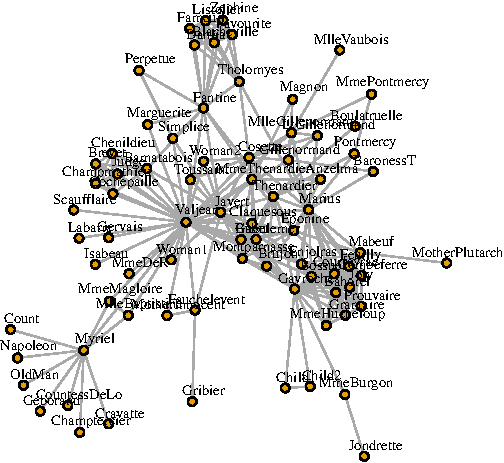
\includegraphics[width=0.6\textwidth]{lesmis.pdf}
	\caption{The \textit{lesmis} dataset.}
	\label{fig:lesmisgraph}
\end{figure*}

As in \cite{wilkinson2017visualizing} we compute the graph-based features centrality, transitivity, closeness, betweenness, degree, average nearest neighbour degree and page rank for each character in the dataset. This transforms the original graph to a rectangular dataset of $77$ observations and $7$ variables, with each observation corresponding to a character in the novel. Figure~\ref{fig:lesmis1} shows the O3 plot for the transformed \textit{lesmis} dataset using the three methods \textit{HDoutliers}, \textit{mvBACON} and \textit{covMCD}. The other three outlier methods used in O3 plots gave computational errors and so could not be used. Figure~\ref{fig:lesmis2} shows the DC1-DC2 space of the transformed \textit{lesmis} dataset.

\begin{figure*}[!ht]
	\centering
	\subfloat[][]{
		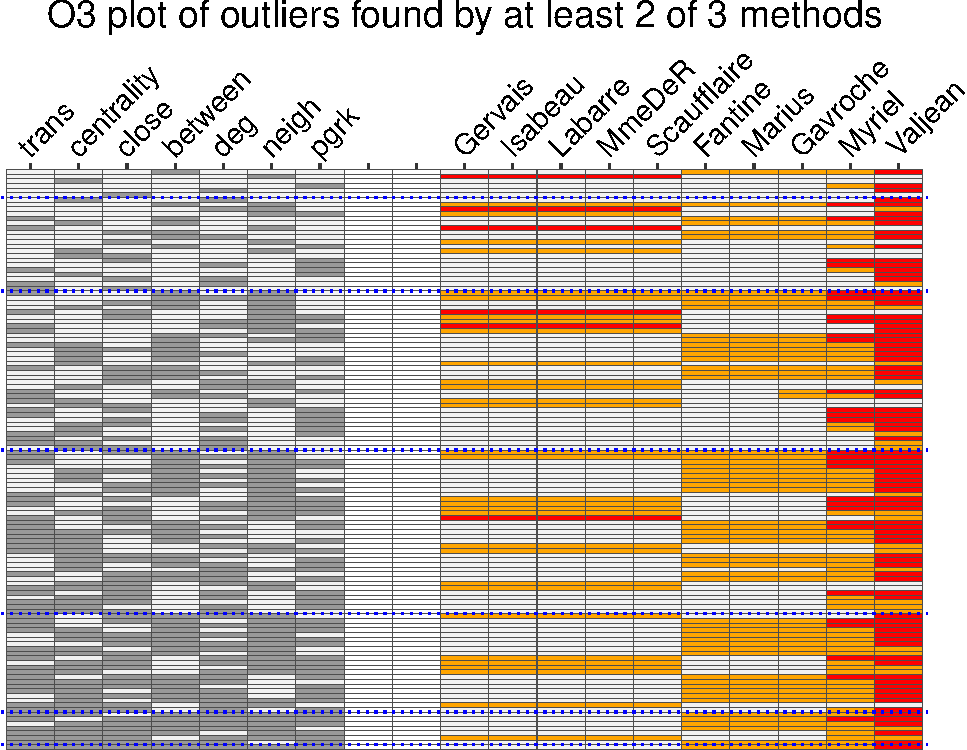
\includegraphics[width=0.54\textwidth]{Ex5_1.pdf}
		\label{fig:lesmis1}
	}\hfill
	\subfloat[][]{
		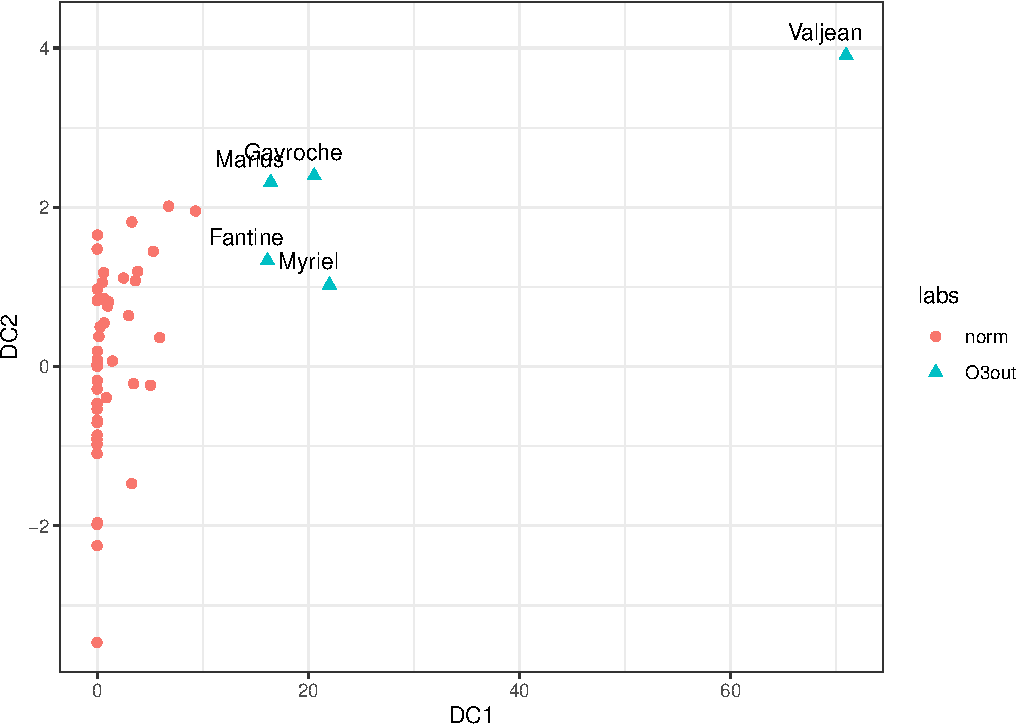
\includegraphics[width=0.43\textwidth]{Ex5_2.pdf}
		\label{fig:lesmis2}
	}%
	\caption{O3plot of the transformed \textit{lesmis} dataset in Figure~\ref{fig:lesmis1} and the first 2 DOBIN components in Figure~\ref{fig:lesmis2}.}
	\label{fig:lesmis}
\end{figure*}

From the O3 plot it is evident that Valjean is the main outlier consistently identified by the three outlier methods in the vast majority of the subspaces. This is confirmed by the DC1-DC2 plot as Valjean appears far away from the rest of the characters in the top right corner. The next most outlying characters in the O3 plot are Myriel, Gavroche, Marius and Fantine. These characters also appear in the DC1-DC2 space somewhat detached from the rest of the characters, although none so remarkably far away as Valjean. A KNN algorithm performed on the first half of the DC components identified Valjean, Myriel, Gavroche, Marius and Fantine as having the highest KNN distances.

As the first DOBIN vector is discriminatory, we look at its coefficients:
The first DOBIN vector has the following coefficients:
\begin{equation}\label{eq:ResWithVis5}
	\text{DC1} = \begin{bmatrix}
		0.0022 & -0.0001 & 0.0032 & 0.9999 & 0.0029 & 0.0025 & 0.0057
	\end{bmatrix}
	\begin{bmatrix}
		\text{Centrality}            \\
		\text{Transitivity}          \\
		\text{Closeness}             \\
		\text{Betweenness}           \\
		\text{Degree}                \\
		\text{Avg. Neighbour Degree} \\
		\text{Page Rank}
	\end{bmatrix} \, .
\end{equation}
From equation~\eqref{eq:ResWithVis5} we see that \textit{Betweenness} is the main feature that makes Valjean an outlier in the DC1-DC2 space. The property \textit{Betweenness} is defined as the number of shortest paths going through a vertex \citep{igraph}. Thus Valjean becomes a node in many shortest paths in the character network making him the main outlier.

\subsection{Classics from Gutenberg}\label{sec:ResWithVis6}

This example is on text analysis of $22$ classics downloaded from the Gutenberg project \citep{gutenberg} and is similar to the example in \cite{wilkinson2017visualizing}. We consider the novels \textit{Alice in Wonderland}, \textit{Anna Karenina}, \textit{Bleak House}, \textit{Emma}, \textit{Frankenstein}, \textit{Gullivers Travels}, \textit{Jude the Obscure}, \textit{Lord Jim}, \textit{Mansfield Park}, \textit{Middlemarch}, \textit{Moby Dick}, \textit{Northanger Abbey}, \textit{Persuasion}, \textit{Pride and Prejudice}, \textit{Sense and Sensibility}, \textit{Silas Marner}, \textit{Sons and Lovers}, \textit{The Life and Opinions of Tristram Shandy}, \textit{Wizard of Oz}, \textit{Ulysses}, \textit{Vanity Fair} and \textit{War and Peace} in our analysis.

We strip each novel into words and obtain the collection of words used and their relative frequencies. This set of words need to be cleaned before computing any useful features. We use the R package \textit{tidytext} \citep{tidytext} for this task. As the first `cleaning' step, we eliminate the stop words such as \textit{the}, \textit{a}, \textit{an} and \textit{in} from our collection. We also remove numbers from our word collection. Next we use a stemming procedure to reduce words to their word stem. For example the words \textit{run} and \textit{running} have the same word stem. This process gives us a cleaned set of words for each novel. We compute the tf-idf (term frequency-inverse document frequency) measure on this collection. The tf-idf statistic measures how important a word is to a document when considering a collection of documents. Consequently we end up with a rectangular dataset of $22$ observations and $39,624$ variables, where each observation is a novel and each variable is the tf-idf statistic of a word.

\begin{figure*}[!hb]
  \centering
  \subfloat[][]{
    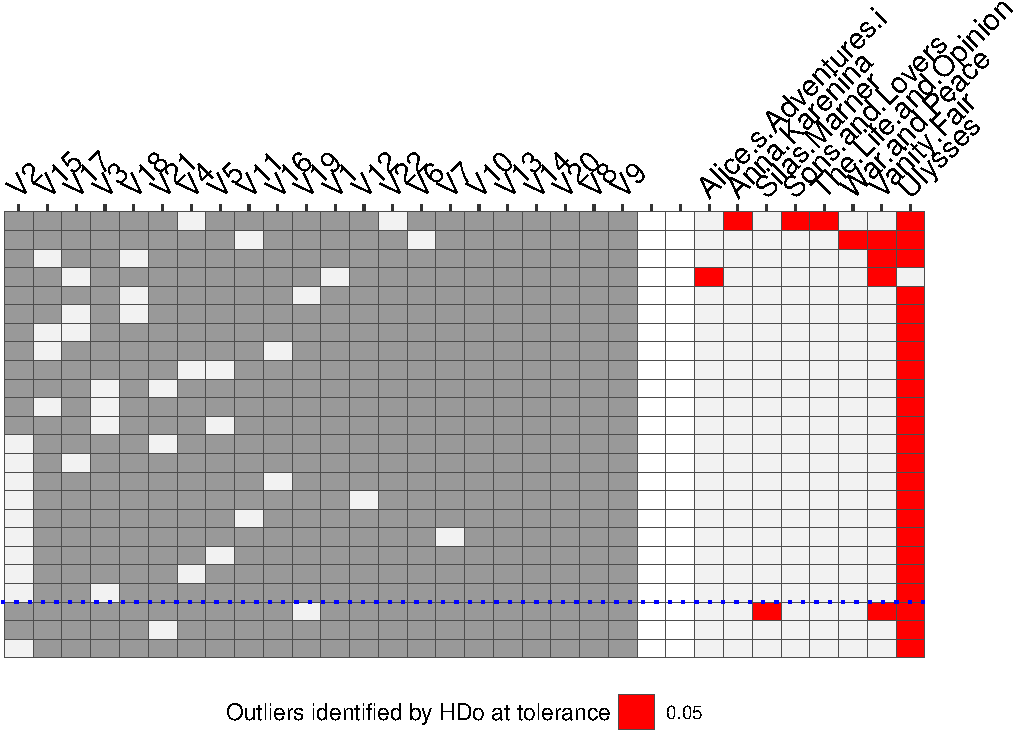
\includegraphics[width=0.54\textwidth]{Ex6_1.pdf}
    \label{fig:gutenberg1}
  }\hfill
  \subfloat[][]{
    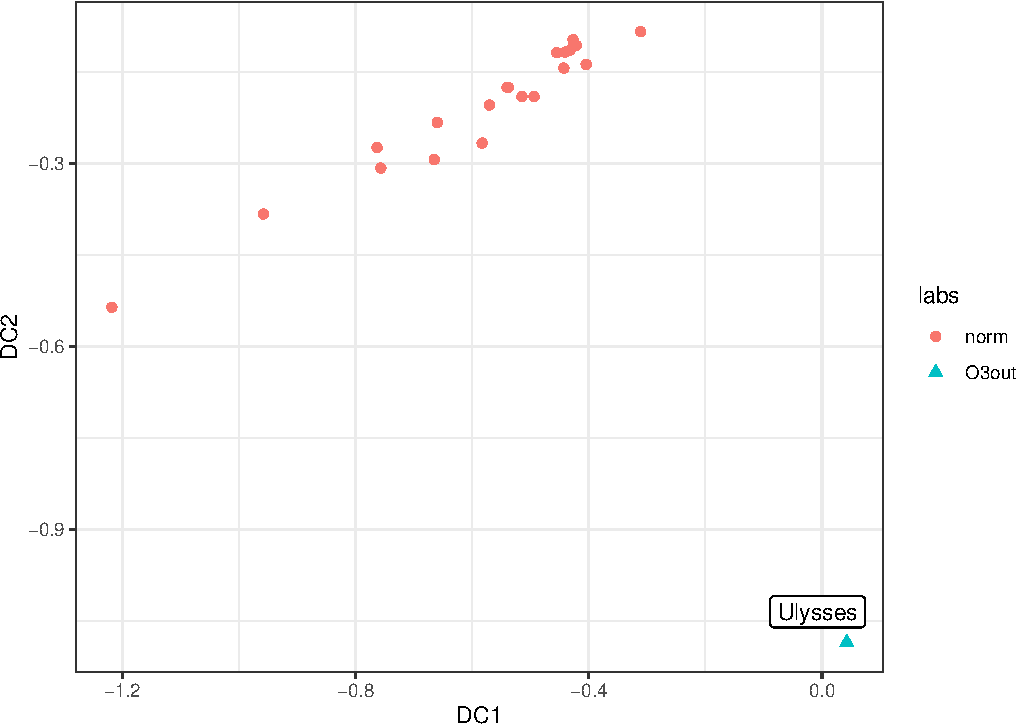
\includegraphics[width=0.43\textwidth]{Ex6_2.pdf}
    \label{fig:gutenberg2}
  }%
  \caption{O3plot of 22 Gutenberg classics in Figure~\ref{fig:gutenberg1} and the first 2 DOBIN components in Figure~\ref{fig:gutenberg2}.}
  \label{fig:gutenberg}
\end{figure*}

However, $22$ vectors in $\mathbb{R}^{39,624}$ can only span a subspace of $22$ dimensions or less. Therefore, we compute this subspace and the respective coordinates of the observations using PCA. We use all the principal components so that we're performing a change of basis and not a projection. As a result we obtain a $22\times 22$ matrix, where each row is an observation corresponding to a novel and each column is a linear combination of $39,624$ tf-idf statistics. The resulting O3 plot using \textit{HDoutliers} and the corresponding DC1-DC2 space is illustrated in Figure~\ref{fig:gutenberg}. Again we see the O3 plot and the DC1-DC2 space agreeing on the most outlying novel \textit{Ulysses} confirming the findings of \cite{wilkinson2017visualizing}. Performing a KNN algorithm yielded \textit{Ulysses} as the observation with the highest KNN distance.

The novel \textit{Ulysses} stands out in the DC1-DC2 space mainly because of its second DC component. However, we do not explore the coefficients of this vector as each coefficient is a linear combination of $39,624$ variables, making it difficult to gain insights.

This section substantiated DOBIN's ability as an outlier visualization tool. In each example we saw the outliers projected onto a 2D space spanned by the first two DOBIN vectors, and their legitimacy was endorsed by the O3 plots. Furthermore, we gained insights about the nature of outlyingness in data by inspecting DOBIN vectors.

% =======================================================================
\section{Results on a data repository}\label{sec:DatRepo}
% =======================================================================

In this section we work with a data repository of $12,642$ datasets \citep{datasets}, generated from approximately $200$ source datasets. Each dataset has labeled outliers and originally was used for classification purposes. The present datasets are modified from its original form by downsampling minority class observations, converting categorical attributes to numerical values, removing missing data and creating several variants from each classification dataset. More details on dataset preparation can be found in \cite{kandanaarachchi2018normalization}. This collection also includes datasets from \cite{campos2016evaluation}.

\todo[inline]{I don't understand the following paragraph. If there is an outlier in a subspace, it is also in the original space by definition. You cannot have outliers that are only in subspaces. \\ Response : changed paragraph beginning. }


A data point that is an outlier in a subspace may not necessarily be an outlier in the full space, specially if other variables drown the subspace outlier \citep{zimek2012survey}. For example in  Figure~\ref{fig:gutenberg1}, the novel \textit{Alice in Wonderland} is an outlier in the fourth subspace in the O3 plot, but not in others.  As we increasingly encounter more  high dimensional data in modern applications, we need to consider it is more likely that certain points are outliers in subspaces rather than in the full input space.  If detecting subspace outliers is a goal, using downsampled classification datasets for outlier detection is sub-optimal. This is because classification datasets generally contain variables that are needed for effective classification, and as a result the labeled outliers in the downsampled dataset may be outliers in the full space. On the other hand, downsampled datasets enable effective evaluation of different pre-processing and outlier methods because they have labeled outliers. Thus, to make these datasets suitable for subspace outlier detection, we ``fatten'' each dataset by adding $20$ noise variables distributed normally, i.e.\ $\sim \mathcal{N}(0,1)$. We use these `fattened' datasets in our experiment.

Similar to Section~\ref{sec:synthetic}, for each dataset we compare the results of three outlier methods LOF, KNN and iForest using the area under the ROC curve (AUC), on three different coordinate systems, namely the full set of coordinates, the first half of the DOBIN components and the first half of the Principal Components. That is, for a dataset with $p$ variables and $N$ observations,  we consider $\lfloor\min(N/2, p/2)\rfloor$ DOBIN and PC components.
%To add to , the datasets are generated from approximately $200$ source datasets. Thus, dataset variants need to be accounted for.

Furthermore, we need to select appropriate tools to present results of $12,642$ datasets across three methods and three coordinate systems. The ability to delve into each dataset and obtain insights is no longer feasible with a large repository. In addition, we want to ascertain whether DOBIN coordinates improve the performance of the three outlier detection methods compared to the other two coordinate systems. Therefore, we investigate each outlier detection method separately. For each outlier method, we compare the performance of the three coordinate systems using a Friedman test adjusting for the dataset variants. To adjust for the dataset variants, we take the median performance for each dataset source and each coordinate system. If the Friedman test is significant, then we perform a Nemenyi test, so that we can rank the coordinate systems according to performance. For convenience we use the shortened names $1/2$ DOBIN for using the first half of DOBIN components, $1/2$ PCA for using the first half of Principal Components and `All Vars' for using all variables in the remainder of the section.

\subsection{Significant tests}\label{sec:DatRepo1}

\todo[inline]{The presentation of results is not clear, and I don't think density plots are the best way of showing them. For each outlier method, we are interested in how the basis set makes a difference. So just show boxplots or simlar of the three sets of AUC results. \\
Response: Changed to boxplots and updated wording.}

Figure~\ref{fig:LOF_FAT} gives the results of the three coordinate systems on outlier detection method LOF. A Friedman test gave the $p$-value $1.986 \times 10^{-5}$, and Figure~\ref{fig:LOF_FAT1} shows the associated Nemenyi plot for this data. This plot shows the ranks of the coordinate systems, with lower ranks indicating better performance. The blue squares highlight methods which are not significantly different from each other. From Figure~\ref{fig:LOF_FAT1} we see that the best coordinates for LOF are $1/2$ DOBIN, followed by $1/2$ PCA and All Vars, with $1/2$ PCA and All Vars not significantly different from each other.
%Figure~\ref{fig:LOF_FAT2} shows the distribution of performance results for LOF using the three coordinate systems. As these curves represent probability density estimates, the area under each curve is $1$. We see that $1/2$ DOBIN components give rise to larger density values for $\text{AUC} > 0.7$, i.e.\ it has a bigger proportion of high AUC values compared to the other two coordinate systems.
Figure~\ref{fig:LOF_FAT2} shows the boxplots for the three coordinate systems. Taking into account that all performance values are roughly between $0.4$ and $1$,  we see that $1/2$ DOBIN has a higher median AUC, and a higher third quartile compared to $1/2$ PCA and All Vars. 

\begin{figure*}[!ht]
	\centering
	\subfloat[][]{
		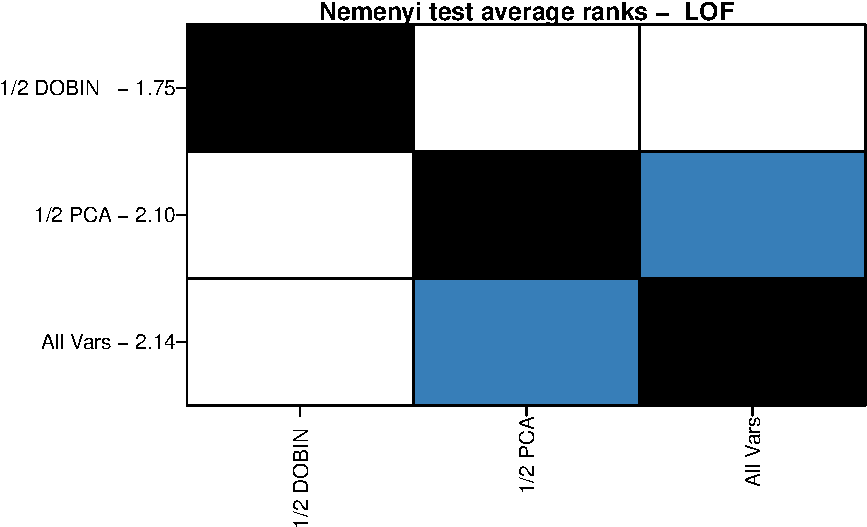
\includegraphics[width=0.48\textwidth]{LOF_Nemenyi_1.pdf}
		\label{fig:LOF_FAT1}
	}\hfill
	\subfloat[][]{
		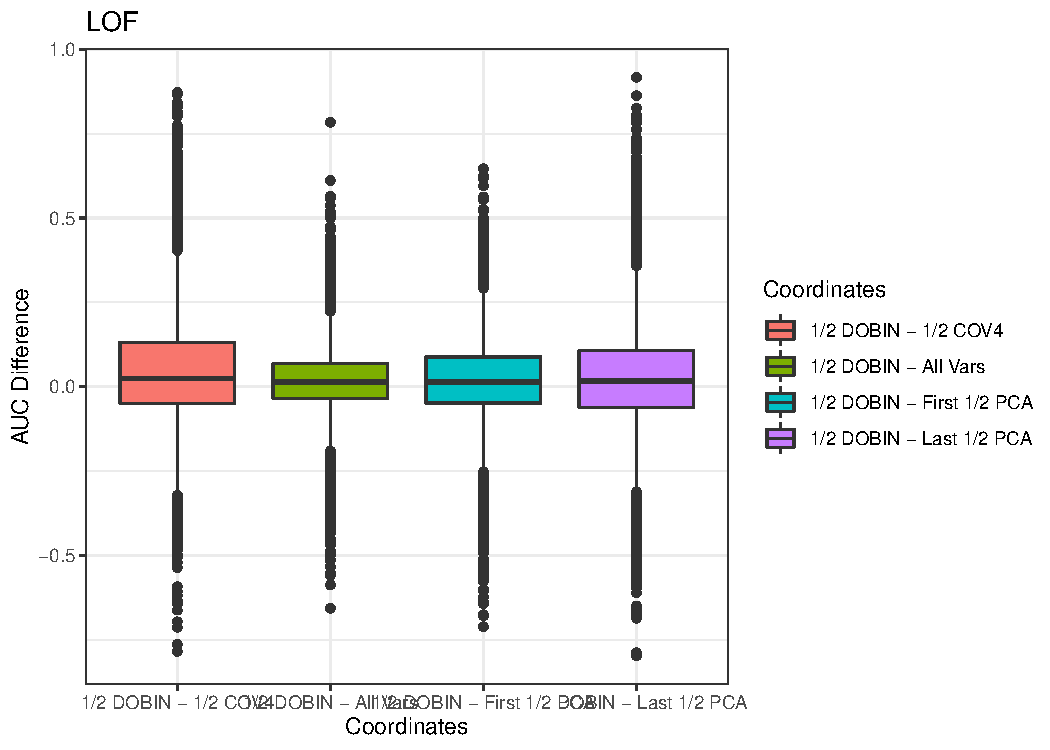
\includegraphics[width=0.48\textwidth]{LOF_BoxPlot.pdf}
		\label{fig:LOF_FAT2}
	}%
	\caption{Nemenyi plot of LOF results on the data repository in Figure~\ref{fig:LOF_FAT1} and the boxplots of the three coordinate systems in Figure~\ref{fig:LOF_FAT2}.}
	\label{fig:LOF_FAT}
\end{figure*}

Figure~\ref{fig:KNN_FAT} shows the results of the three coordinate systems on the outlier detection method KNN. We obtained the $p$-value $1.341\times 10^{-8}$ from the Friedman test. Again, from Figure~\ref{fig:KNN_FAT1} we see that $1/2$ DOBIN outperforms All Vars and $1/2$ PCA, which is corroborated by the boxplot in Figure~\ref{fig:KNN_FAT2}. Even though All Vars is ranked second, it is not significantly different from $1/2$ PCA for KNN.

\begin{figure*}[!ht]
	\centering
	\subfloat[][]{
		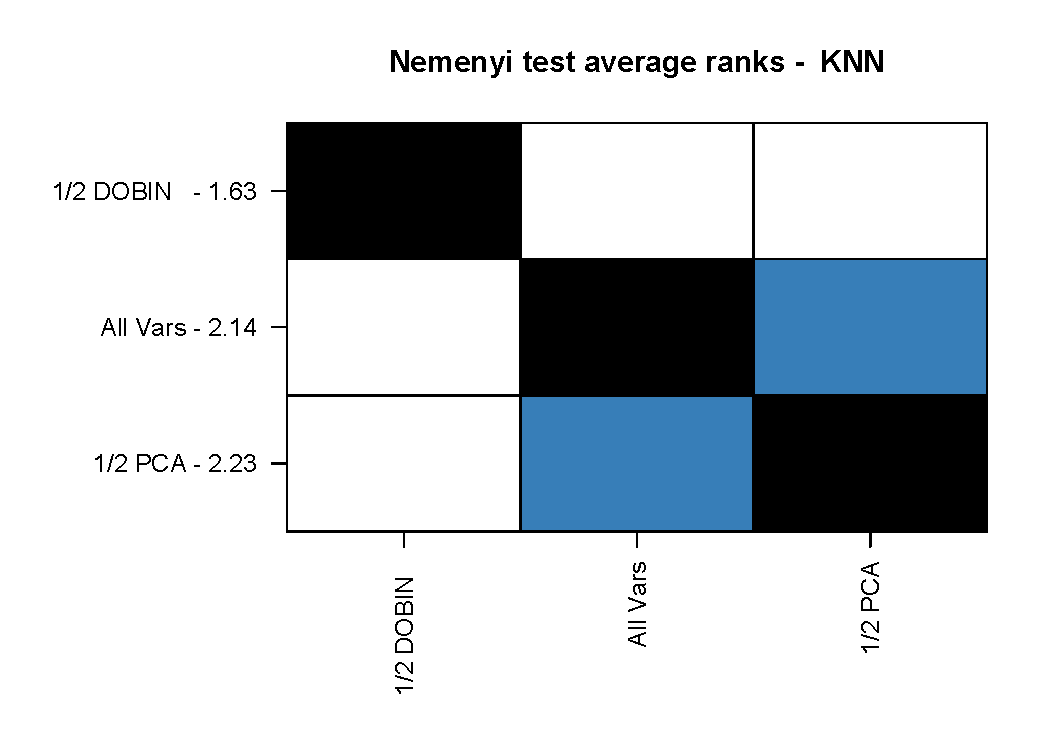
\includegraphics[width=0.48\textwidth]{KNN_Nemenyi_1.pdf}
		\label{fig:KNN_FAT1}
	}\hfill
	\subfloat[][]{
		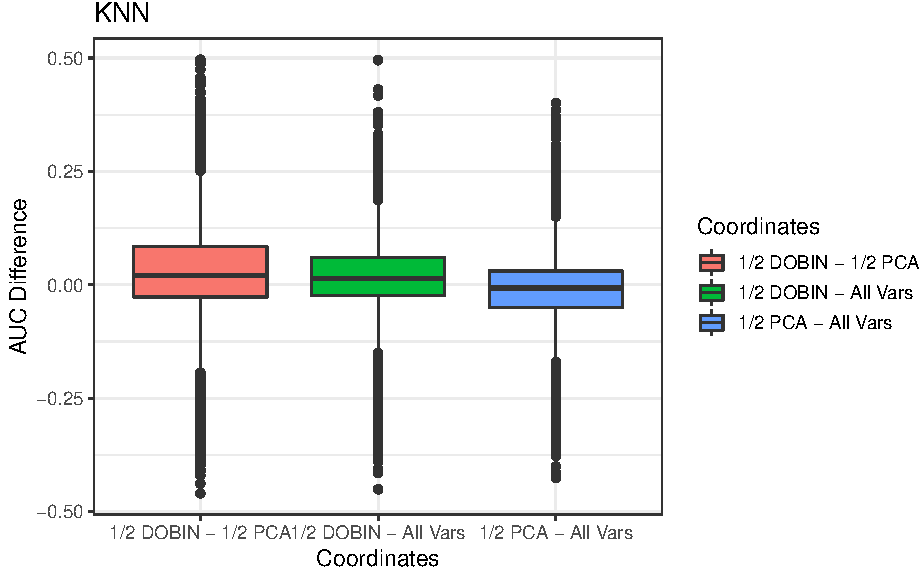
\includegraphics[width=0.48\textwidth]{KNN_BoxPlot.pdf}
		\label{fig:KNN_FAT2}
	}%
	\caption{Nemenyi plot of KNN results on the data repository in Figure~\ref{fig:KNN_FAT1} and the boxplots of the three coordinate systems in Figure~\ref{fig:KNN_FAT2}.}
	\label{fig:KNN_FAT}
\end{figure*}

Similar performances are obtained for iForest, which is illustrated in Figure~\ref{fig:IFOREST_FAT}. A Friedman test conducted on the data gave a $p$-value less than $2.2 \times 10^{-16}$. The Nemenyi plot shows that while $1/2$ DOBIN performs the best, all three methods are significantly different from each other, with All Vars outperforming $1/2$ PCA. This is supported from the boxplots in Figure~\ref{fig:IFOREST_FAT2}, with $1/2$ DOBIN having a higher median and third quartile compared to others. 

%the curve associated to $1/2$ DOBIN lying above the All Vars curve, and the All Vars curve lying above $1/2$ PCA curve for $\text{AUC} > 0.65$.

\begin{figure*}[!ht]
	\centering
	\subfloat[][]{
		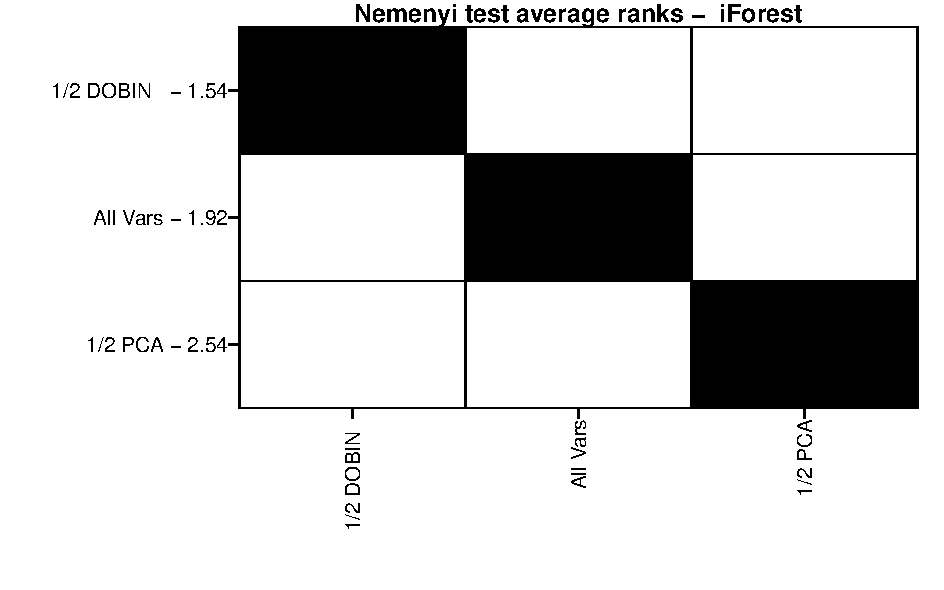
\includegraphics[width=0.48\textwidth]{IFOREST_Nemenyi_1.pdf}
		\label{fig:IFOREST_FAT1}
	}\hfill
	\subfloat[][]{
		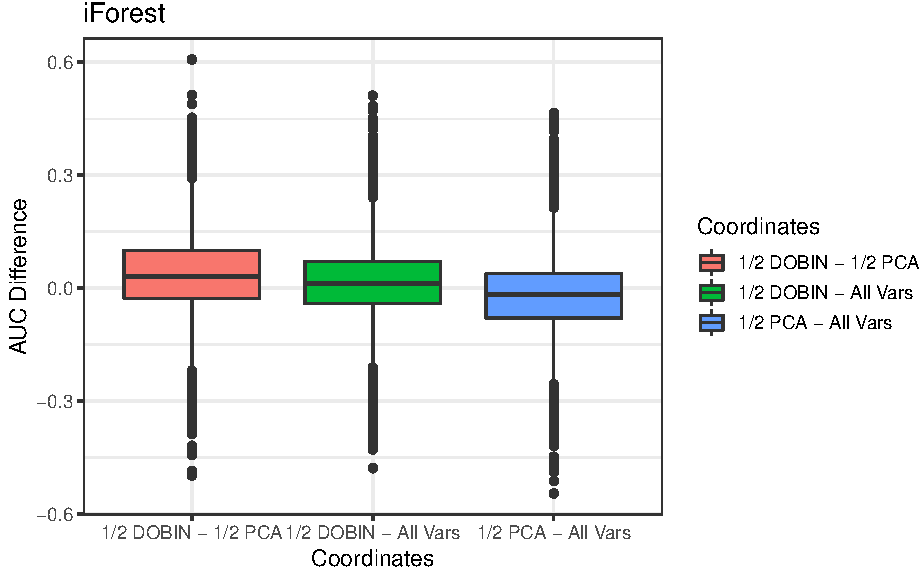
\includegraphics[width=0.48\textwidth]{IFOREST_BoxPlot.pdf}
		\label{fig:IFOREST_FAT2}
	}%
	\caption{Nemenyi plot of iForest results on the data repository in Figure~\ref{fig:IFOREST_FAT1} and the boxplots of the three coordinate systems in Figure~\ref{fig:IFOREST_FAT2}.}
	\label{fig:IFOREST_FAT}
\end{figure*}

We see that $1/2$ DOBIN performs best for all three outlier detection methods and is significantly better than $1/2$ PCA and All Vars. This is evidence that DOBIN is better as a dimension reduction tool for outier detection compared to PCA and the original variables. We attribute this success to DOBIN's firm mathematical foundations.

% =======================================================================
\section{Conclusion}
% =======================================================================

Dimension reduction for outlier detection is a topic that has not received much attention in the literature. One way to achieve this is to construct a basis that empowers outlier detection. In this paper, we present DOBIN: a Distance based Outlier BasIs using Neighbours, which strives to accomplish this goal. We used DOBIN on an extensive data repository of real world datasets and showed that DOBIN basis improves performance of the outlier detection methods LOF, KNN and iForest. Using half of the DOBIN components we outperformed PCA and the standard basis as coordinate systems for these three outlier detection methods.

In addition, we conducted a visual analysis of outliers using DOBIN on six datasets from diverse sources, which included a character graph from the novel \textit{Les Mis\'erables} and $22$ classics from Gutenberg website. We projected the data onto a 2D space spanned by the first two DOBIN vectors, and saw that outliers identified by many methods in O3 plots were indeed far away from the rest of the data. We gained insights about the outliers in these datasets, and identified the variables that contributed to make them outliers.

\todo[inline]{A rotation invariant form would be PCA first followed by DOBIN. You lose the interpretability but gain on rotation-invariance. I think we should say this here \\
Response :  added these comments. }

Currently DOBIN is sensitive to rotations in the input space. As future work we plan to investigate avenues that can contribute to a rotation invariant version of DOBIN. A rotation invariant form would give the same results if PCA was performed before DOBIN. Even though we gain rotation-invariance from such a version, we lose the interpretablity of results by performing an arbitrary rotation.  However, rotation-invariance may be advantageous for working with datasets that are already pre-processed.   The R package \textit{dobin} contains the implementation and is available at \url{https://github.com/sevvandi/dobin} for download.

% =======================================================================
\subsection*{Supplementary Material}
% =======================================================================

\textbf{R package dobin}: This package contains the DOBIN basis construction.

\textbf{Datasets}: Datasets discussed in Section~\ref{sec:DatRepo} are available at \cite{datasets}. The character network from the novel \textit{Les Mis\'erables} was taken from the R package \textit{SOMbrero} \citep{sombrero}. The book vectors dataset used in Section~\ref{sec:ResWithVis6} is available at the github repository \url{https://github.com/sevvandi/Outlier-Basis}.

\textbf{Scripts}: The script \texttt{Figures\_For\_Paper\_1.R} contains the R code used to conduct experiments and produce graphs in Section~\ref{sec:synthetic}. The script \texttt{Figures\_For\_Paper\_2.R} contains the R code used in Section~\ref{sec:ResWithVis}. And finally, the script \texttt{Figures\_For\_Paper\_3.R} contains the R code used to produce the graphs in Section~\ref{sec:DatRepo}. The original computation on the data repository detailed in Section~\ref{sec:DatRepo} was conducted using the MonARCH HPC Cluster. The results of this computation are available at the github repository \url{https://github.com/sevvandi/Outlier-Basis}.

\textbf{Other R-packages}: In addition to the R package \textit{dobin} we have also used the R packages \textit{OutliersO3} \citep{O3Rpack}, \textit{isolationForest} \citep{isolationForest}, \textit{DMwR} \citep{DMwR}, \textit{pROC} \citep{pROC}, \textit{ggplot2} \citep{ggplot2}, \textit{mbgraphic} \citep{mbgraphic}, \textit{gridExtra} \citep{gridextra}, \textit{tsutils} \citep{tsutils}, \textit{tidyverse} \citep{tidyverse} and \textit{tidyr} \citep{tidyr}.%\todo{Suggest you replace reshape2 with tidyr. This is not recommended these days.}


% =======================================================================
\subsection*{Acknowledgements}
% =======================================================================

Funding was provided by the Australian Research Council through the Linkage Project LP160101885. This research was also supported by the Monash eResearch Centre and eSolutions-Research Support Services through the MonARCH HPC Cluster.

% =======================================================================
\bibliographystyle{agsm} %Choose a bibliograhpic style
\bibliography{Master}
% =======================================================================
\end{document}
